\documentclass[12pt,a4paper]{article}

\usepackage{kotex}
\usepackage{amsmath,amssymb,amsfonts}
\usepackage{graphicx}
\usepackage{textcomp}
\usepackage{xcolor}
\usepackage{booktabs}
\usepackage{multirow}
\usepackage{url}
\usepackage{array}
\usepackage{enumitem}
\usepackage{balance}
\usepackage[margin=2.5cm]{geometry}
\usepackage{hyperref}
\usepackage{listings}
\graphicspath{{../../figures/}}

\lstdefinestyle{pseudocode}{
  basicstyle=\ttfamily\small,
  frame=single,
  columns=fullflexible,
  keepspaces=true,
  showstringspaces=false,
  xleftmargin=0.5em,
  xrightmargin=0.5em
}

\begin{document}

\title{\textbf{TA-BRPL: Trust-Aware Backpressure RPL}\\
\large Blackhole + Sinkhole 복합 공격 환경에서의\\
온-노드 신뢰 모델 설계, 구현 및 검증\\[0.5em]
\normalsize 연구 노트 v0.4.0 (최종 수정: 2026-03-27)}

\author{TA-BRPL Research Group\\
Contiki-NG / Cooja 기반 구현}

\maketitle
\tableofcontents
\newpage

% ============================================================
\begin{abstract}
% ============================================================

TA-BRPL(Trust-Aware Backpressure RPL)은 저전력 손실 네트워크(LLN)에서
backpressure 기반 혼잡 인식 라우팅과 온-노드 신뢰 관리를 결합한 프로토콜이다.
기반이 되는 BRPL(Backpressure RPL)의 목적 함수에 세 가지 신뢰 성분,
즉 $T_\text{fwd}$(포워딩 신뢰), $T_\text{ctrl}$(제어 평면 신뢰),
$T_\text{hon}$(혼잡 정직성 신뢰)을 직접 결합하며,
별도의 2단계 검증 모델이 하드 격리(blacklist) 결정을 독립적으로 담당한다.

v0.4.0에서는 sinkhole 중심 2-시나리오 실험
(Sinkhole-only / Sinkhole+Drop50, $2\times2\times2\times5=40$ runs)을
정식 반영하였다. 또한 decision policy를
``신규 parent 채택(admission) 억제 강화 + 기존 parent 유지/탈출 신중화''로 재구성하였다.
최신 policy v3 결과에서 TA-BRPL은 baseline(v0.3.x 설정) 대비
churn을 크게 줄이면서, Sinkhole+Drop50 구간에서
GRID의 PDR(0.768$\rightarrow$0.801), attacker share(0.165$\rightarrow$0.147),
hit ratio(0.200$\rightarrow$0.147)를 개선했고,
BOTTLE에서도 PDR(0.738$\rightarrow$0.745), attacker share(0.149$\rightarrow$0.122),
hit ratio(0.263$\rightarrow$0.188) 개선을 보였다.
다만 BRPL 절대 성능 대비 격차가 남아 있어,
본 문서는 이를 ``policy refinement stage''로 명시한다.

본 문서는 TA-BRPL의 모든 구성 요소, 설계 의도, 구현 세부 사항,
동작 원리, 실험 설정 및 결과를 한국어로 총정리한 기술 참조 문서이다.
본 버전(v0.4.0)은 고정 GRID 중심 결과에 더해
GRID/BOTTLE 비교 스윕 결과와 정책 변경 이력을 함께 포함한다.

\textbf{키워드:} IoT, LLN, RPL, BRPL, 신뢰 관리, Blackhole 공격,
Sinkhole 공격, 선택적 포워딩, Cooja, Contiki-NG
\end{abstract}

% ============================================================
\section*{v0.4.0 업데이트 요약}
% ============================================================
\addcontentsline{toc}{section}{v0.4.0 업데이트 요약}

\begin{itemize}
  \item \textbf{평가 프레임 갱신}: Sinkhole-only / Sinkhole+Drop50 2시나리오,
  GRID/BOTTLE 2토폴로지, BRPL/TA-BRPL 2프로토콜, seed 5개(총 40-run).
  \item \textbf{정책 축 재정의}: ``soft suspicion vs hard evidence'' 계층을 유지하면서,
  \textbf{신규 parent admission 억제}를 직접 강화하고
  기존 parent 유지/탈출은 보수적으로 운영.
  \item \textbf{정책 v3 성과}: baseline 대비 churn 재악화 없이
  attacker dependency(att\_share, hit\_ratio)와 during PDR의 동시 개선을 확인.
\end{itemize}

\begin{table}[h]
  \centering
  \caption{Sinkhole+Drop50에서 policy v3 vs baseline (TA-BRPL)}
  \label{tab:v040_policy_v3}
  \begin{tabular}{lcccc}
    \toprule
    Topology & PDR$_\text{dur}$ & att\_share & hit\_ratio & churn \\
    \midrule
    GRID   & 0.768 $\rightarrow$ \textbf{0.801} & 0.165 $\rightarrow$ \textbf{0.147} & 0.200 $\rightarrow$ \textbf{0.147} & 2.1 $\rightarrow$ \textbf{0.6} \\
    BOTTLE & 0.738 $\rightarrow$ \textbf{0.745} & 0.149 $\rightarrow$ \textbf{0.122} & 0.263 $\rightarrow$ \textbf{0.188} & 2.7 $\rightarrow$ \textbf{0.8} \\
    \bottomrule
  \end{tabular}
\end{table}

% ============================================================
\section{연구 목표와 설계 철학}
% ============================================================

\subsection{연구 동기}

LLN 환경에서의 라우팅 공격은 두 가지 형태로 대별된다.
첫째, \textbf{Blackhole 공격}은 노드가 라우팅 프로토콜에 정상 참여하면서
IP 계층에서 전달해야 할 패킷을 선택적으로 드롭한다.
MAC 계층의 ACK는 정상 전달되므로 상위 계층에서는 탐지가 어렵다.
둘째, \textbf{Sinkhole 공격}은 노드가 DIO(DODAG Information Object) 메시지의
rank 필드를 비정상적으로 낮게 광고하여 인근 노드들을 자신을 통해 라우팅하도록
유인하고, 유입된 트래픽을 드롭하는 방식이다.

기존 신뢰 관리 접근법의 한계는 크게 두 가지다.
\begin{enumerate}
  \item \textbf{forwarding rate 기반 감시의 한계}: 혼잡으로 패킷을 드롭하는 정직한 노드와
  의도적으로 드롭하는 공격자를 forwarding rate만으로는 구분할 수 없다.
  \item \textbf{Trust floor 문제}: 가중합 기반 trust 모델에서
  일부 성분이 환경 상수로 고정되면, trust의 최솟값이 탐지 임계값 위에 묶여
  공격자가 배제되지 않는다. (SMTrust의 구조적 한계, Section~\ref{sec:smtrust} 참조)
\end{enumerate}

\subsection{설계 목표}

TA-BRPL은 다음 목표를 동시에 만족하도록 설계되었다.
\begin{itemize}
  \item \textbf{G1}: BRPL이 제공하는 backpressure 기반 혼잡 인식 라우팅 능력을 유지한다.
  \item \textbf{G2}: Blackhole 및 sinkhole에 대해 노드 내 자율적 탐지 및 우회 능력을 제공한다.
  \item \textbf{G3}: 정상 노드에 대한 과오탐(false positive)과 과패널티를 최소화한다.
  \item \textbf{G4}: 기존 RPL-Classic 소스를 직접 수정하지 않고,
  weak-symbol 오버라이드 방식으로 결합하여 모듈성을 확보한다.
\end{itemize}

\subsection{설계 원칙}

\begin{itemize}
  \item \textbf{에코 기반 end-to-end 확인}: 단순 도청(overhearing)이 아닌
  root의 에코 응답을 통해 패킷이 실제로 root까지 도달했는지 확인한다.
  \item \textbf{혼잡과 공격의 분리}: $T_\text{hon}$을 통해 혼잡으로 인한 forwarding 저하와
  의도적 드롭을 구분한다.
  \item \textbf{비대칭 EWMA}: 공격 탐지 반응은 빠르게, 신뢰 회복은 느리게 설정하여
  on-off 공격 전략을 억제한다.
  \item \textbf{2단계 검증}: trust EWMA와 독립적인 누적 증거 기반 검증 모델로
  하드 격리 결정을 보수적으로 내린다.
\end{itemize}

% ============================================================
\section{전체 시스템 아키텍처}
% ============================================================

\subsection{계층 구조}

TA-BRPL은 Contiki-NG의 RPL-Classic 라우팅 스택 위에서 동작한다.
전체 소프트웨어 계층 구조는 다음과 같다.

\begin{center}
\begin{tabular}{|c|}
\hline
\textbf{사용자 프로세스 (sender.c, receiver\_root.c)} \\
\hline
\textbf{TA-BRPL 신뢰 엔진 (ta-brpl-trust.c/h)} \\
\hline
\textbf{BRPL 목적 함수 (rpl-brpl.c)} ← weak-symbol 오버라이드 \\
\hline
\textbf{RPL-Classic 라우팅 스택 (Contiki-NG)} \\
\hline
\textbf{IPv6/UDP/MAC 스택} \\
\hline
\end{tabular}
\end{center}

핵심 구현 파일은 \texttt{ta-brpl-trust.c/h}이며,
BRPL의 목적 함수(\texttt{rpl-brpl.c})가 trust 정보를 요청할 때
C언어의 weak-symbol 메커니즘을 통해 TA-BRPL의 구현이 자동으로 호출된다.
이 설계 덕분에 TA-BRPL 모듈을 컴파일에서 제외하더라도
RPL-Classic 및 BRPL의 원본 소스를 수정할 필요가 없다.

\subsection{정보 흐름}

trust 엔진으로 입력되는 이벤트는 다음 세 경로를 통해 전달된다.

\begin{enumerate}
  \item \textbf{에코 응답 훅 (\texttt{echo\_rx\_callback})}:
  sender.c에서 root로 UDP 패킷을 전송할 때 현재 preferred parent를
  \texttt{remember\_tx\_parent(seq, parent\_id)}로 기록한다.
  root가 패킷을 수신하면 에코 응답을 발신자에게 반환하고,
  에코 수신 시 \texttt{take\_tx\_parent(seq)}로 해당 parent를 역추적하여
  \texttt{ta\_trust\_notify\_forwarded(parent\_id)}를 호출한다.
  이를 통해 에코 기반 포워딩 관찰값 $F_{ij}$를 갱신한다.

  \item \textbf{IP 입력 훅 (\texttt{ta\_ip\_input\_hook})}:
  Contiki-NG의 \texttt{NETSTACK\_IP\_PACKET\_PROCESSOR} 훅을 통해
  수신된 패킷 중 RPL DIO 메시지(ICMPv6, code=0x02)를 파싱하여
  $T_\text{ctrl}$ 지표(rank/version/frequency 이상)를 갱신한다.

  \item \textbf{BRPL 큐 콜백}:
  RPL parent table에서 이웃 노드의 BRPL 큐 광고값($Q_\text{adv}$, $Q_\text{max}$)을
  주기적으로 읽어 $T_\text{hon}$ 계산에 사용한다.

  \item \textbf{Parent 교체 콜백 (\texttt{RPL\_CALLBACK\_PARENT\_SWITCH})}:
  \texttt{project-conf.h}에서 \texttt{RPL\_CALLBACK\_PARENT\_SWITCH}를
  \texttt{brpl\_parent\_switch\_callback}으로 정의하여,
  preferred parent 교체 시 \texttt{brpl\_preferred\_parent\_changed()}가 호출된다.
  이를 통해 \texttt{current\_parent\_id}와 escape 타이머를 갱신한다.
  이 훅이 없으면 escape 메커니즘은 발동하지 않는다.
\end{enumerate}

trust 엔진에서 BRPL 목적 함수로 제공하는 출력 인터페이스:

\begin{itemize}
  \item \texttt{brpl\_trust\_get(node\_id)}: trust EWMA 값 [0, 1000] 반환
  \item \texttt{brpl\_penalty\_scale\_get(node\_id)}: 신뢰 기반 동적 패널티 배율 반환
  \item \texttt{brpl\_validation\_penalty\_scale\_get(node\_id)}: 검증 모델 기반 패널티 배율 반환
  \item \texttt{brpl\_escape\_mode\_get(node\_id)}: escape 모드 활성 여부 반환
  \item \texttt{brpl\_trust\_parent\_allowed(node\_id)}: parent 후보 허용 여부 반환
\end{itemize}

\begin{figure}[t]
  \centering
  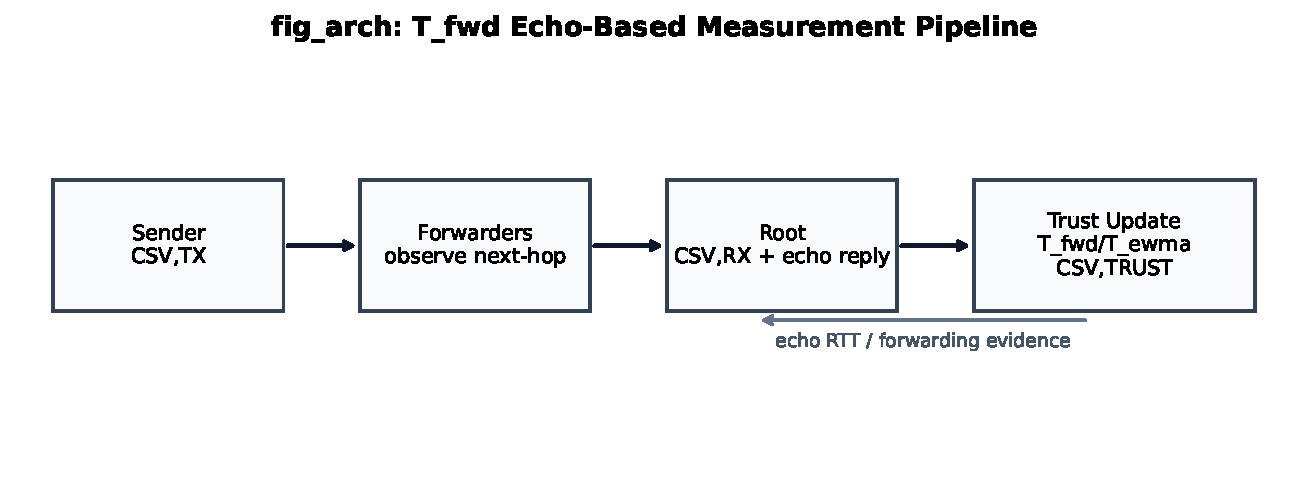
\includegraphics[width=\linewidth]{fig_arch_system_flow.pdf}
  \caption{TA-BRPL 시스템 정보 흐름도. sender가 패킷을 전송하면
  parent ID가 기록되고, root의 에코 응답 수신 시 해당 parent의 $T_\text{fwd}$가 갱신된다.
  DIO 수신은 IP 입력 훅에서 파싱되어 $T_\text{ctrl}$에 반영된다.}
  \label{fig:arch_flow}
\end{figure}

\subsection{파라미터 단일 소스 정책}

모든 tunable 파라미터는 \texttt{project-conf.h}의 C 매크로로 정의된다.
각 프로토콜 변형의 \texttt{Makefile.*}은 모드 플래그(\texttt{TABRPL\_MODE=1} 등)만 설정하며,
임계값, $\lambda$ 값, 패널티 배율 등은 모두 \texttt{project-conf.h}에서 집중 관리된다.
민감도 실험은 컴파일러 커맨드라인에서 특정 매크로만 오버라이드하는 방식으로 수행된다.

% ============================================================
\section{신뢰 성분 상세 설명}
% ============================================================

\subsection{$T_\text{fwd}$: 포워딩 신뢰 (Forwarding Trust)}
\label{sec:tfwd}

$T_\text{fwd}(i,j)$는 노드 $i$의 관점에서 이웃 $j$가 패킷을
신뢰성 있게 root까지 전달하는지를 측정하는 성분이다.

\subsubsection{에코 기반 end-to-end 측정 원리}

\paragraph{왜 도청(overhearing)이 아닌 에코 기반인가?}

초기 버전에서는 IEEE 802.15.4 채널에서 이웃 노드가 다음 홉으로 패킷을
전달하는 순간을 수동으로 도청(passive overhearing)하여 $T_\text{fwd}$를 측정하였다.
그러나 802.15.4 unicast 통신에서 CSMA 드라이버는 자신에게 주소되지 않은 프레임을
MAC 계층에서 폐기한다. 따라서 진정한 상향 포워딩 이벤트를 도청하는 것은
물리적으로 불가능하다. 더 나아가, 하향 경로(root $\to$ sender)의 에코 응답이
parent를 거쳐 오는 경우 이를 포워딩 증거로 잘못 인식하면
선택적 포워딩 공격자에게 \emph{거짓 양성} 포워딩 점수를 부여할 수 있다.

에코 기반 방식은 이 두 문제를 모두 해결한다.
패킷이 실제로 root까지 도달했는지를 root의 에코 응답으로 확인하므로,
IP 계층 선택적 드롭을 MAC 투명하게 탐지할 수 있다.

\paragraph{동작 흐름}

\begin{enumerate}
  \item 노드 $i$가 이웃 $j$를 preferred parent로 하여 데이터 패킷(seq=$s$)을 전송할 때,
  \texttt{ta\_trust\_notify\_sent(j)}를 호출하여 카운터 $S_{ij}$를 1 증가시킨다.
  동시에 \texttt{remember\_tx\_parent(s, j)}로 seq--parent 쌍을 환형 버퍼에 기록한다.

  \item Root가 해당 패킷을 수신하면 발신자에게 에코 응답(``seq=$s$ t0=$t$'')을 반환한다.

  \item 발신자가 에코를 수신하면 \texttt{echo\_rx\_callback}이 호출된다.
  \texttt{take\_tx\_parent(s)}로 해당 seq를 전송했던 parent $j$를 역추적하고,
  \texttt{ta\_trust\_notify\_forwarded(j)}를 호출하여 $F_{ij}$를 1 증가시킨다.
\end{enumerate}

\paragraph{의사코드 (구현 참조: \texttt{sender.c}, \texttt{ta-brpl-trust.c})}
\begin{lstlisting}[style=pseudocode]
on_data_send(seq, parent_id):
  ta_trust_notify_sent(parent_id)      # S_ij++
  remember_tx_parent(seq, parent_id)   # ring buffer

on_echo_receive(seq):
  parent_id = take_tx_parent(seq)
  if parent_id != 0:
    ta_trust_notify_forwarded(parent_id)  # F_ij++

on_trust_window_update(neighbor j):
  if fwd_sent_new(j) == 0:
    tfwd = prr_from_etx_or_fallback(j)    # PRR fallback
  else:
    expected = fwd_sent_new(j) * prr_from_etx_or_fallback(j)
    tfwd = (fwd_observed_new(j) + alpha) / (expected + alpha + beta)
  tfwd = clamp_scale(tfwd, 0, 1000)
\end{lstlisting}

\paragraph{수식}

Laplace smoothing 파라미터 $(\alpha, \beta)$를 적용한 포워딩 성공률:
\begin{equation}
  T_\text{fwd}^{(raw)}(i,j) = \frac{F_{ij} + \alpha}{E_{ij} + \alpha + \beta},
  \quad E_{ij} = S_{ij} \cdot \hat{P}_\text{RR}(j)
  \label{eq:tfwd_raw}
\end{equation}
여기서 $E_{ij}$는 링크 손실을 고려한 기대 포워딩 횟수이고,
$\hat{P}_\text{RR}(j)$는 MAC 계층 ETX로부터 추정한 패킷 수신률(PRR)이다.
$\alpha = \beta = 1$로 Laplace 스무딩을 적용하여 초기 관찰에서
trust가 0 또는 1로 급격히 치우치는 것을 방지한다.

\subsubsection{PRR 폴백: 부트스트래핑 메커니즘}
\label{sec:prr_fallback}

에코 기반 측정의 근본적 한계는 에코 회신이 하향 경로(root $\to$ sender)의
수렴을 필요로 한다는 점이다.
DODAG 형성 초기에는 DAO가 root에 도달하지 않아 하향 경로가 개통되지 않으며,
실측 에코 도달률은 약 7\%에 불과하다.

이 상태에서 방치하면 다음 사망 나선(death spiral)이 발생한다.
\begin{align*}
  S_{ij} &\nearrow \text{(패킷 전송마다 증가)} \\
  F_{ij} &= 0 \text{(에코가 도달하지 않음)} \\
  T_\text{fwd} &= \frac{0+1}{S_{ij}+2} \to 0 \text{(S 누적으로 붕괴)}
\end{align*}
trust EWMA가 $\tau_\text{join} = 350$ 미만으로 하락하면 모든 parent가
후보 집합에서 제외되어 라우팅이 완전히 붕괴된다.

이를 방지하기 위해, 현재 update window에서 새로운 전송이 없는 경우
(\texttt{fwd\_sent\_new == 0}) 링크 통계 ETX로부터 추정한 PRR을
$T_\text{fwd}$의 대안 값으로 사용한다.

\begin{equation}
  T_\text{fwd}(i,j) =
  \begin{cases}
    \hat{P}_\text{RR}(j) & \text{fwd\_sent\_new} = 0 \text{ (PRR 폴백)} \\[6pt]
    T_\text{fwd}^{(raw)}(i,j) & \text{fwd\_sent\_new} > 0 \text{ (에코 기반)}
  \end{cases}
  \label{eq:tfwd_switch}
\end{equation}

\paragraph{PRR 추정 방법}

Contiki-NG의 link-stats 모듈이 관리하는 ETX(Expected Transmission Count)로부터:
\begin{equation}
  \hat{P}_\text{RR}(j) = \text{clamp}\!\left(
    \frac{\texttt{LINK\_STATS\_ETX\_DIVISOR}}{ETX_j},\;
    P_\text{min},\; P_\text{max}
  \right)
  \label{eq:prr}
\end{equation}
ETX 통계가 아직 충분하지 않은 경우(\texttt{link\_stats\_is\_fresh} 미달)에는
$P_\text{fallback} = 1000$(lossless 가정)을 사용한다.

\paragraph{fwd\_sent\_new 조건의 의미}

\texttt{fwd\_sent\_new}는 현재 update window에서 새롭게 전송한 패킷 수이며,
매 업데이트 주기 후 0으로 리셋된다(하프닝 없음).
이를 조건으로 사용하는 이유는 다음 두 경우를 정확히 구분하기 위해서이다.

\begin{itemize}
  \item \textbf{이번 창에 전송이 없는 경우} (\texttt{fwd\_sent\_new}=0):
  현재 parent로 사용되지 않는 이웃이므로 에코 증거가 없는 것은 당연하다.
  PRR 폴백을 사용하여 통신 품질 기반 trust를 유지한다.
  이 경우는 부트스트래핑뿐만 아니라 경로 변동(route churn) 이후
  이전 parent가 일시적으로 비활성화된 경우도 포함된다.

  \item \textbf{이번 창에 전송이 있으나 에코가 없는 경우} (\texttt{fwd\_sent\_new}$>0$, $F_{ij}^{(new)}=0$):
  패킷이 전송되었으나 root에 도달하지 않은 전형적인 blackhole 시그니처이다.
  에코 기반 수식을 적용하면 $T_\text{fwd}$가 낮아져 공격자 탐지로 이어진다.
\end{itemize}

이전 구현에서 \texttt{fwd\_observed\_new == 0}을 조건으로 사용했을 때의 문제점:
공격자는 항상 \texttt{fwd\_observed\_new}가 0이었으므로 PRR 폴백을 받아
$T_\text{fwd} \approx 1000$을 유지하고, 오히려 정직한 노드(에코 70\% 도달률)가
낮은 $T_\text{fwd} \approx 700$을 가지는 역전 현상이 발생하였다.
\texttt{fwd\_sent\_new}를 조건으로 변경하여 이 문제를 해결하였다.

\subsubsection{카운터 감쇠: 할빙(halving) 방식}

매 업데이트 주기($\Delta t = 60$초)마다 누적 카운터를 우측 비트시프트로 반감한다.
\begin{equation}
  S_{ij} \leftarrow S_{ij} \gg 1,\quad F_{ij} \leftarrow F_{ij} \gg 1
\end{equation}

완전 리셋(zeroing) 대신 할빙을 사용하는 이유는, 리셋 시 공격자가
잠시(한 window 동안) 정상 동작을 보이는 것만으로 $T_\text{fwd}$가 다시
중립값(500)으로 초기화되어 trust가 회복되는 on-off 공격 취약점이 발생하기 때문이다.
할빙을 통해 과거 관찰의 영향이 지수적으로 감쇠하면서도 완전히 사라지지 않아,
약 2$\sim$3 업데이트 창의 유효 메모리를 유지한다.

\subsubsection{T\_fwd 날카로움(sharpening)}

옵션으로 \texttt{TA\_TFWD\_SHARPEN\_SCALE} 파라미터를 1000 초과로 설정하면
$T_\text{fwd}$를 중립값(500) 기준으로 확장하여 honest/attacker 간 차이를 증폭한다.
현재 기본값은 1000으로 비활성화 상태이다.

\subsection{$T_\text{ctrl}$: 제어 평면 신뢰 (Control-Plane Trust)}
\label{sec:tctrl}

$T_\text{ctrl}$은 이웃 노드의 RPL 제어 메시지 동작에서
이상 징후를 탐지하는 성분이다.
IP 입력 훅에서 DIO ICMPv6 메시지(type=155, code=0x02)를 파싱하여
기본 3개 이상 지표($A_\text{rank}, A_\text{DIO}, A_\text{ver}$)와
지속 저-rank 유인 지표($A_\text{lure}$)를 갱신한다.

\subsubsection{Rank 이상 지표 ($A_\text{rank}$)}

\begin{itemize}
  \item \textbf{절대 이상}: DIO에 포함된 rank가 root rank($= \texttt{min\_hoprankinc}$)보다
  낮은 경우. 물리적으로 불가능한 값이므로 rank 이상 카운터를 즉시 증가시킨다.
  이는 sinkhole이 rank=128(또는 더 낮은 값)을 광고하여 root보다 더 좋은 경로를
  주장하는 공격을 탐지한다.

  \item \textbf{과도한 rank 감소}: 동일한 DODAG version 번호를 유지하면서
  rank가 \texttt{min\_hoprankinc / 2} 이상 감소하는 경우.
  실제 링크 품질 개선으로 인한 rank 변동(ETX 기반)과 구별하기 위해
  hysteresis 임계값(\texttt{min\_hoprankinc / 2})을 적용한다.
\end{itemize}

\subsubsection{DIO 빈도 이상 지표 ($A_\text{DIO}$)}

Trickle 타이머 기반의 정상 DIO 전송률(\texttt{TA\_TRUST\_DIO\_NORMAL\_RATE} = 5회/창)
대비 과도한 DIO 전송은 DIO flooding 또는 trickle 억제 공격의 신호로 해석한다.
\begin{equation}
  A_\text{DIO} = \frac{\max(0,\; \texttt{ctrl\_dio\_count} - N_\text{normal})}{\texttt{ctrl\_dio\_count}}
\end{equation}

\subsubsection{Version 이상 지표 ($A_\text{ver}$)}

Root에서 전파되지 않은 RPL DODAG version 번호의 증가는
강제 DODAG 재시작을 유발하는 version attack의 신호이다.
동일 version 맥락에서 rank가 급감하면 rank 이상으로 처리하고,
version이 변경되면 새 baseline으로 업데이트하여 합법적인 DODAG 재시작을 허용한다.

\subsubsection{지속 저-rank 유인 지표 ($A_\text{lure}$)}

sinkhole은 root 근처 rank를 반복 광고하여 신규 parent 채택을 유도한다.
v0.4.0에서는 이 패턴을 직접 반영하기 위해
``low-rank streak''와 ``low-rank count''를 별도로 누적한다.
동일 DODAG version에서 near-root rank 광고가 연속적으로 관찰되면
$A_\text{lure}$를 증가시키고, 시간이 지나면 할빙(decay)으로 완만히 감쇠시킨다.

\subsubsection{가중합 + lure 보정 집계}

\begin{equation}
  A_{ij}^{(\text{base})} =
  \frac{w_1 \cdot A_\text{rank} + w_2 \cdot A_\text{DIO} + w_3 \cdot A_\text{ver}}{10}
\end{equation}
\begin{equation}
  A_{ij} = \min\!\left(1,\; A_{ij}^{(\text{base})} + \kappa_\text{lure}\cdot A_\text{lure}\right)
\end{equation}
\begin{equation}
  T_\text{ctrl}(i,j) = 1 - A_{ij}
\end{equation}
기본 가중치: $w_1=5$ (rank), $w_2=3$ (DIO), $w_3=2$ (version).
\(\kappa_\text{lure}\)는 low-rank 유인 보정 강도(코드에서는 penalty scale 상수)이다.

카운터는 매 업데이트 주기마다 할빙되어 과거 이상의 영향이 시간에 따라 감쇠한다.
데이터가 없는 경우($\texttt{ctrl\_dio\_count}=0$) $A_x=0$을 적용하여
$T_\text{ctrl}=1.0$을 유지한다.

\paragraph{의사코드 (구현 참조: \texttt{ta\_ip\_input\_hook})}
\begin{lstlisting}[style=pseudocode]
on_dio_rx(neighbor j, rank, version):
  ctrl_dio_count[j] += 1

  if rank < root_rank:
    rank_anomaly[j] += 1
  else if same_version(j, version) and rank_drop_too_fast(j, rank):
    rank_anomaly[j] += 1

  if version_jump_without_root(j, version):
    ver_anomaly[j] += 1

on_window_update_ctrl(j):
  A_rank = normalize(rank_anomaly[j], ctrl_dio_count[j])
  A_dio  = max(0, ctrl_dio_count[j] - dio_normal_rate) / max(1, ctrl_dio_count[j])
  A_ver  = normalize(ver_anomaly[j], ctrl_dio_count[j])
  A_lure = normalize(low_rank_lure_count[j], ctrl_dio_count[j])
  A_base = (5*A_rank + 3*A_dio + 2*A_ver) / 10
  A = min(1, A_base + k_lure*A_lure)
  tctrl = 1000 * (1 - A)
  halve_ctrl_counters(j)
\end{lstlisting}

\subsection{$T_\text{hon}$: 혼잡 정직성 신뢰 (Congestion-Honesty Trust)}
\label{sec:thon}

$T_\text{hon}$은 이웃 $j$가 자신의 큐 상태를 정직하게 광고하는지를
검증하는 성분이다. 이 성분의 핵심 목적은 혼잡과 공격을 분리하는 것이다.

\paragraph{동작 원리}

BRPL 프로토콜에서 각 노드는 DIO 메시지에 현재 큐 점유율($Q_\text{adv}$)과
최대 큐 크기($Q_\text{max}$)를 실어 보낸다.
노드 $i$는 자신의 로컬 큐 상태를 이용하여 이웃 $j$의 예상 큐 점유율($Q_\text{est}$)을 추정하고,
광고값과 추정값의 차이를 기반으로 정직성을 평가한다.

\begin{equation}
  Q_\text{est}(j) = \frac{q_\text{local}}{q_{\max,\text{local}}} \cdot Q_{\max}(j)
\end{equation}

\begin{equation}
  T_\text{hon}(i,j) = 1 - \min\!\left(1,\;
  \frac{|Q_\text{adv}(j) - Q_\text{est}(j)|}{Q_{\max}(j)}\right)
  \label{eq:thon}
\end{equation}

\paragraph{혼잡과 공격의 구분}

정직하게 혼잡한 노드는 $Q_\text{adv}(j) \approx Q_\text{est}(j)$를 만족하므로
$T_\text{hon} \approx 1.0$을 유지한다. 반면 공격자가 혼잡하지 않음에도
낮은 큐 점유율을 허위 광고하면 두 값의 차이가 커져 $T_\text{hon}$이 감소한다.

초기 데이터가 없는 경우(\texttt{hon\_valid}=0) $T_\text{hon}=1.0$으로 초기화하여
미지 노드에게 이익의 여지를 준다.

\paragraph{의사코드 (구현 참조: BRPL queue 광고 파싱 경로)}
\begin{lstlisting}[style=pseudocode]
on_queue_advertisement(neighbor j, q_adv, q_max):
  q_est = (local_q / local_q_max) * q_max
  diff  = abs(q_adv - q_est)
  thon  = 1 - min(1, diff / max(1, q_max))
  if have_valid_queue_obs(j):
    trust_hon[j] = scale1000(thon)
  else:
    trust_hon[j] = 1000
\end{lstlisting}

\subsection{가중 기하평균 집계}
\label{sec:aggregate}

세 trust 성분은 가중 기하평균으로 결합되어 최종 신뢰 관찰값 $\tilde{T}$를 산출한다.

\begin{equation}
  \tilde{T}(i,j) =
  \left(\frac{T_\text{fwd}}{S}\right)^{w_f/W} \cdot
  \left(\frac{T_\text{ctrl}}{S}\right)^{w_c/W} \cdot
  \left(\frac{T_\text{hon}}{S}\right)^{w_h/W} \cdot S
  \label{eq:aggregate}
\end{equation}

여기서 $S = \texttt{TA\_TRUST\_SCALE} = 1000$은 정수 연산 스케일,
$W = w_f + w_c + w_h = 10$, 기본 가중치 벡터는 $(w_f, w_c, w_h) = (5, 3, 2)$이다.
구현상으로는 glibc의 \texttt{pow()} 함수를 사용하여 부동소수점으로 계산 후
정수로 변환한다.

\paragraph{기하평균 사용의 이유}

산술평균과 달리 기하평균에서는 어느 한 성분이라도 0에 가까워지면
전체 trust가 크게 하락한다. 이는 공격자가 특정 지표(예: $T_\text{ctrl}$, $T_\text{hon}$)만
정상적으로 유지하면서 $T_\text{fwd}$만 조작하는 전략으로 높은 신뢰를
유지하기 어렵게 만든다.

\paragraph{순수 Blackhole의 기하평균 Floor 문제}

그러나 순수 blackhole 공격자는 $T_\text{ctrl} \approx 1000$,
$T_\text{hon} \approx 1000$을 유지하므로, $T_\text{fwd}$가 아무리 낮아도
기하평균의 최솟값은 다음과 같이 제한된다.
\begin{equation}
  \tilde{T}_\text{min} = T_\text{fwd}^{0.5} \cdot 1000^{0.5}
  = \sqrt{T_\text{fwd} \cdot 1000}
\end{equation}
예를 들어 $T_\text{fwd} = 167$이면 $\tilde{T}_\text{min} \approx 408$이며,
$\tau_\text{join} = 350$을 충족하므로 기하평균만으로는 배제 불가능하다.
이 문제를 해결하기 위해 독립 $T_\text{fwd}$ EWMA(\texttt{trust\_fwd})가 도입되었다.
(Section~\ref{sec:trust_fwd_ewma} 참조)

\subsection{비대칭 EWMA 업데이트}
\label{sec:ewma}

매 $\Delta t = 60$초마다 per-neighbor trust를 다음 점화식으로 업데이트한다.

\begin{equation}
  T_{ij}(t+1) = \lambda(t)\, T_{ij}(t) + (1-\lambda(t))\, \tilde{T}_{ij}
  \label{eq:ewma}
\end{equation}

\begin{equation}
  \lambda(t) =
  \begin{cases}
    \lambda_\downarrow = 0.4 & \tilde{T}_{ij} < T_{ij}(t) \quad \text{(신뢰 하락 시)} \\
    \lambda_\uparrow   = 0.7 & \text{otherwise} \quad \text{(신뢰 유지/회복 시)}
  \end{cases}
  \label{eq:lambda}
\end{equation}

\paragraph{비대칭 설계 의도}

\begin{itemize}
  \item $\lambda_\downarrow = 0.4$ (신규 관찰 가중치 60\%):
  공격 시작 후 2$\sim$3 업데이트 창(120$\sim$180초)에 걸쳐 trust를
  $\tau_\text{join}$ 이하로 하락시켜 공격자 배제 달성.
  이전에 0.2를 사용했을 때 FP 과다 문제가 발생하였으므로 0.4로 조정하였다.

  \item $\lambda_\uparrow = 0.7$ (신규 관찰 가중치 30\%):
  trust 회복을 의도적으로 늦춰, 공격자가 잠시 정상 동작을 보이며
  trust를 빠르게 회복하는 on-off 공격 전략에 대응한다.
\end{itemize}

\paragraph{의사코드 (구현 참조: \texttt{ta\_trust\_update\_all})}
\begin{lstlisting}[style=pseudocode]
on_window_update(neighbor j):
  tfwd  = compute_tfwd(j)
  tctrl = compute_tctrl(j)
  thon  = compute_thon(j)

  t_obs = geo_mean_weighted(tfwd, tctrl, thon, wf=5, wc=3, wh=2)

  if t_obs < trust[j]:
    lambda_main = 0.4
  else:
    lambda_main = 0.7
  trust[j] = ewma(trust[j], t_obs, lambda_main)

  if tfwd < trust_fwd[j]:
    lambda_fwd = 0.2
  else:
    lambda_fwd = 0.7
  trust_fwd[j] = ewma(trust_fwd[j], tfwd, lambda_fwd)
\end{lstlisting}

\subsection{독립 $T_\text{fwd}$ EWMA: \texttt{trust\_fwd}}
\label{sec:trust_fwd_ewma}

Section~\ref{sec:aggregate}에서 설명한 기하평균 floor 문제를 해결하기 위해,
집계 trust EWMA(\texttt{trust})와 별개로 포워딩 신뢰만의 독립 EWMA인
\texttt{trust\_fwd}를 추적한다.

\begin{equation}
  \texttt{trust\_fwd}_{ij}(t+1) = \lambda_\text{fwd}(t) \cdot \texttt{trust\_fwd}_{ij}(t)
  + (1-\lambda_\text{fwd}(t)) \cdot T_\text{fwd}(i,j)
\end{equation}

이때 $\lambda_\text{fwd}$는 감소 시 $\texttt{TA\_TRUST\_LAMBDA\_DECREASE\_FWD} = 0.2$를
사용하여(집계 EWMA의 $\lambda_\downarrow = 0.4$보다 빠른 반응),
blackhole 탐지 신호인 $T_\text{fwd}$의 하락을 신속하게 반영한다.

\texttt{trust\_fwd}는 검증 모델의 판단 보조 신호로도 사용되며,
escape 트리거 조건과 지속 패널티 조건에서도 참조된다.

% ============================================================
\section{검증 모델 (Validation Model)}
% ============================================================
\label{sec:validation}

검증 모델은 trust EWMA와 독립적으로 동작하는 2단계 증거 누적 시스템으로,
하드 격리(blacklist) 결정을 보수적으로 내리기 위해 설계되었다.
trust EWMA는 60초마다 업데이트되어 빠른 패널티 반응을 제공하지만,
단일 업데이트 창의 변동에 민감할 수 있다.
검증 모델은 장기 누적 증거를 기반으로 하여 오탐(FP)을 억제한다.

\subsection{검증 상태 (Review State)}

각 이웃 노드에 대해 세 가지 검증 상태가 유지된다.

\begin{center}
\begin{tabular}{lll}
\toprule
상태 & 심벌 & 의미 \\
\midrule
\texttt{TA\_REVIEW\_STATE\_NORMAL}    & 0 & 정상, 패널티 없음 (배율 1.0$\times$) \\
\texttt{TA\_REVIEW\_STATE\_UNDER}     & 1 & 의심, 경량 패널티 (배율 1.6$\times$) \\
\texttt{TA\_REVIEW\_STATE\_PENALIZED} & 2 & 강한 증거, 중패널티 (배율 2.2$\times$) \\
\bottomrule
\end{tabular}
\end{center}

blacklist된 노드는 검증 패널티 배율 3.0$\times$를 받는다.

\subsection{리뷰 스코어 시스템}

검증 창(review window)은 다음 조건이 모두 성립할 때 활성화된다.
\begin{itemize}
  \item 현재 이웃이 preferred parent이다 (\texttt{node\_id == current\_parent\_id}).
  \item 현재 창에서 최소 \texttt{TA\_TRUST\_VALIDATION\_MIN\_SENT}(=3)회 이상 전송.
  \item 현재 parent로 선택된 지 \texttt{TA\_TRUST\_VALIDATION\_MIN\_PARENT\_AGE\_SECONDS}(=120초) 이상 경과.
\end{itemize}

검증 창이 활성화되면 누적 전송 횟수(\texttt{val\_sent\_acc})와
에코 관찰 횟수(\texttt{val\_obs\_acc})를 기반으로 성공률을 계산한다.

\begin{equation}
  \text{success\_pm} = \frac{\texttt{val\_obs\_acc}}{\texttt{val\_sent\_acc}} \times 1000
\end{equation}

성공률에 따라 세 가지 신호 중 하나가 판정된다.
\begin{itemize}
  \item \textbf{bad\_signal}: \texttt{val\_sent\_acc} $\ge$ 8이고
  성공률 $\le$ 150 (15\% 미만). 리뷰 스코어 +3.
  \item \textbf{strong\_bad}: \texttt{val\_sent\_acc} $\ge$ 10이고
  성공률 $\le$ 100 (10\% 미만). 추가 보너스 스코어 +2.
  \item \textbf{good\_signal}: \texttt{val\_sent\_acc} $\ge$ 8이고
  성공률 $\ge$ 550 (55\% 이상). 리뷰 스코어 $-2$.
\end{itemize}

검증 창이 비활성인 경우(parent가 아니거나 전송이 적은 경우):
리뷰 스코어 $-1$, \texttt{val\_sent\_acc}/\texttt{val\_obs\_acc} 절반 감쇠.

\subsection{상태 전환 조건}

\begin{itemize}
  \item 리뷰 스코어 $\ge$ \texttt{TA\_TRUST\_REVIEW\_SCORE\_PENALIZED}(=14) $\to$ PENALIZED 상태
  \item 리뷰 스코어 $\ge$ \texttt{TA\_TRUST\_REVIEW\_SCORE\_UNDER}(=8) $\to$ UNDER 상태
  \item 그 외 $\to$ NORMAL 상태
\end{itemize}

별도의 blacklist 트리거: \texttt{strong\_bad} 신호가
\texttt{TA\_TRUST\_VALIDATION\_BAD\_STREAK\_FOR\_BLACKLIST}(=1)회 이상 연속으로
발생하고 스코어가 \texttt{TA\_TRUST\_REVIEW\_SCORE\_BLACKLIST}(=7) 이상이면
blacklist 처리된다.

\paragraph{의사코드 (구현 참조: \texttt{ta\_validation\_update\_review})}
\begin{lstlisting}[style=pseudocode]
update_validation(neighbor j):
  review_active =
    is_current_parent(j) and
    sent_new(j) >= MIN_SENT and
    parent_age(j) >= MIN_PARENT_AGE

  if review_active:
    sent_acc[j] += sent_new(j)
    obs_acc[j]  += obs_new(j)
    success_pm = 1000 * obs_acc[j] / max(1, sent_acc[j])

    bad_signal    = (sent_acc[j] >= 8  and success_pm <= 150)
    strong_bad    = (sent_acc[j] >= 10 and success_pm <= 100)
    good_signal   = (sent_acc[j] >= 8  and success_pm >= 550)

    if bad_signal:  review_score[j] += 3
    if strong_bad:  review_score[j] += 2; strong_bad_streak[j] += 1
    else:           strong_bad_streak[j] = 0
    if good_signal: review_score[j] -= 2
  else:
    review_score[j] -= 1
    sent_acc[j] >>= 1
    obs_acc[j]  >>= 1
    strong_bad_streak[j] = 0

  review_score[j] = clamp(review_score[j], 0, SCORE_MAX)
  review_state[j] = score_to_state(review_score[j])

  if strong_bad_streak[j] >= BAD_STREAK_FOR_BLACKLIST and
     review_score[j] >= SCORE_BLACKLIST:
    blacklist(j)
\end{lstlisting}

\subsection{검증 패널티 배율}

\texttt{brpl\_validation\_penalty\_scale\_get(node\_id)} 함수는 검증 상태에 따라
다음 배율을 반환한다. BRPL 목적 함수는 이 배율을 routing cost에 곱하여
의심 노드를 라우팅 후보 선호도에서 후순위로 밀어낸다.

\begin{equation}
  P_\text{val}(\text{state}) =
  \begin{cases}
    3000 & \text{BLACKLISTED} \\
    2200 & \text{PENALIZED} \\
    1600 & \text{UNDER} \\
    1000 & \text{NORMAL}
  \end{cases}
\end{equation}

\paragraph{검증모델 데이터 가시화}
최신 30-seed 로그에서 검증모델 이벤트를 별도로 집계해 시각화하였다.
Figure~\ref{fig:val_events}는 검증 상태 전이/blacklist 이벤트의 클래스별 빈도를,
Figure~\ref{fig:val_cum}는 blacklist 누적 시점을, Figure~\ref{fig:val_nodes}는
blacklist가 집중된 이웃 ID 분포를 보여준다.

\begin{figure}[t]
  \centering
  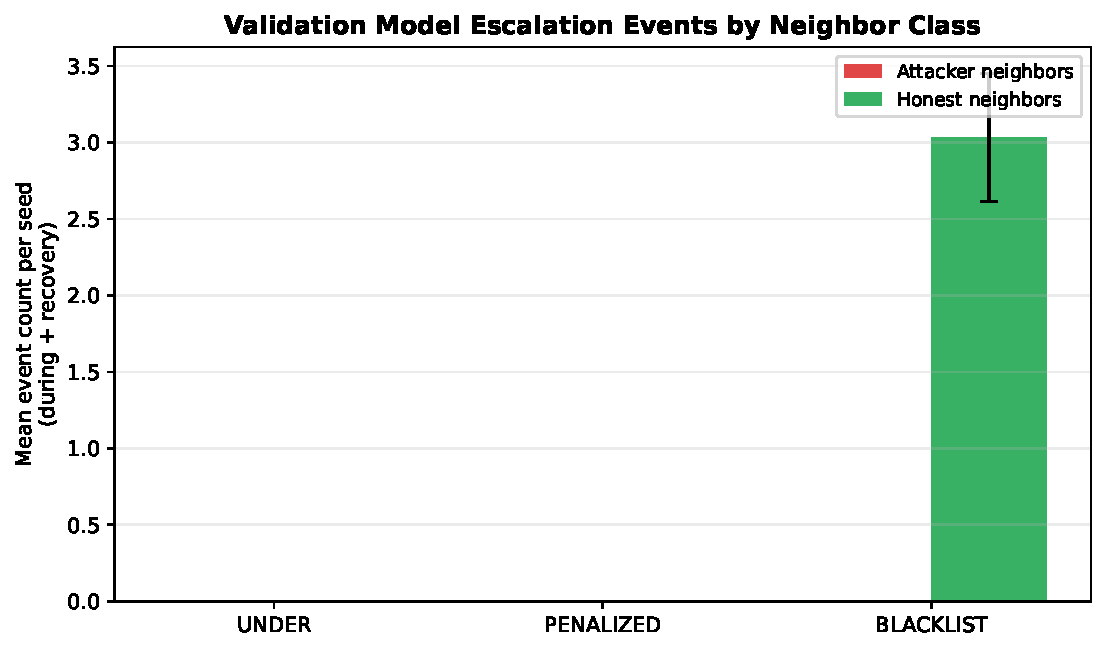
\includegraphics[width=\linewidth]{fig_validation_events.pdf}
  \caption{검증모델 이벤트(UNDER/PENALIZED/BLACKLIST) 빈도.
  현재 실험에서는 상태 전이 이벤트보다 blacklist 이벤트가 지배적으로 관찰된다.}
  \label{fig:val_events}
\end{figure}

\begin{figure}[t]
  \centering
  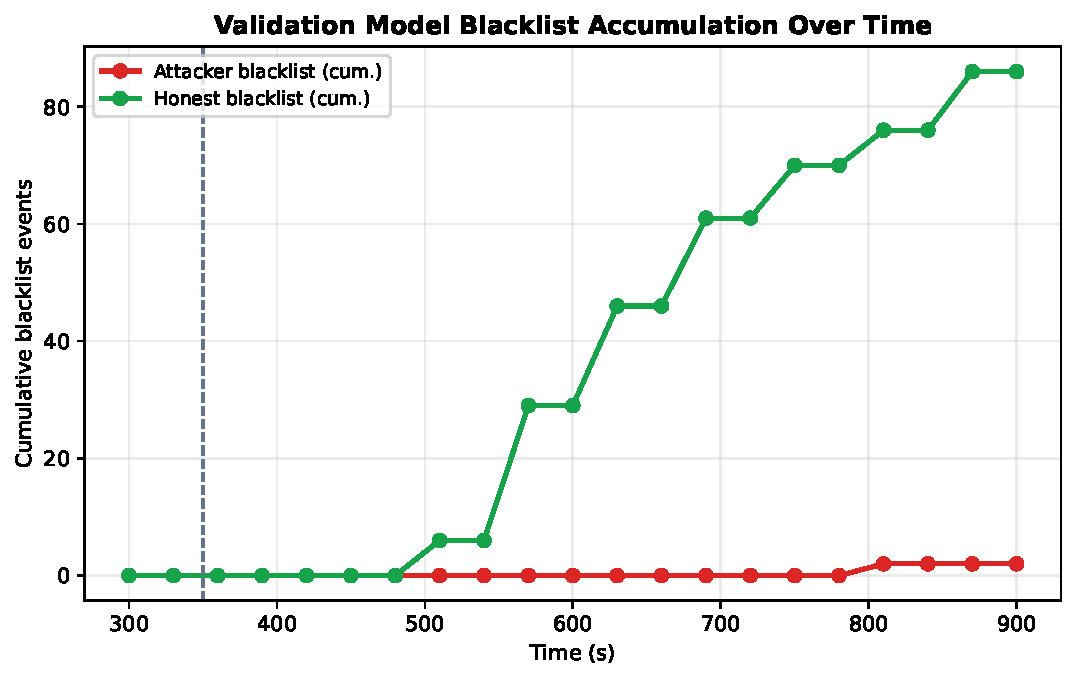
\includegraphics[width=\linewidth]{fig_validation_cumulative.pdf}
  \caption{검증모델 blacklist 누적 시계열(공격기 이후).
  공격 구간 이후 blacklist 이벤트가 단계적으로 누적되는 양상을 보인다.}
  \label{fig:val_cum}
\end{figure}

\begin{figure}[t]
  \centering
  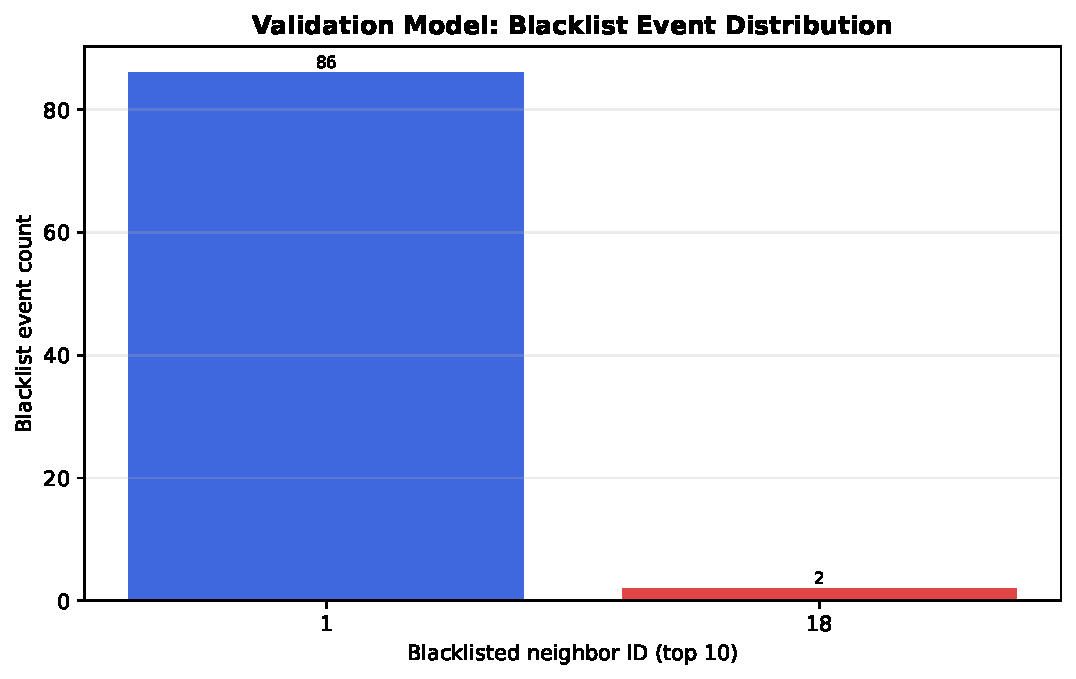
\includegraphics[width=\linewidth]{fig_validation_blacklist_nodes.pdf}
  \caption{검증모델 blacklist 대상 이웃 ID 분포(top 10). 재실험 로그 기준
  node 1(루트 경유 경로)과 node 18(sinkhole 인접)에 이벤트가 집중된다.}
  \label{fig:val_nodes}
\end{figure}

% ============================================================
\section{임계값 정책, 패널티 및 격리 메커니즘}
% ============================================================

\subsection{3단계 임계값 정책}

trust EWMA 값 $T_{ij} \in [0, 1000]$은 세 임계값에 의해 네 tier로 분류된다.

\begin{table}[h]
  \centering
  \caption{TA-BRPL trust tier 정의}
  \label{tab:thresholds}
  \begin{tabular}{lllp{6cm}}
    \toprule
    Tier & 범위 & 상태 & 효과 \\
    \midrule
    Normal    & $T \ge 600$ & NORMAL
      & 패널티 없음. BRPL cost 변경 없음 \\
    Suspect   & $350 \le T < 600$ & SUSPECT
      & cost 배율 패널티 적용. parent 후보로는 허용 \\
    Untrusted & $200 \le T < 350$ & UNTRUSTED
      & parent 후보 사실상 제외 (cost 매우 높음) \\
    Blacklist & $T < 200$ & BLACKLISTED
      & 120초 하드 격리. parent 후보에서 완전 제외 \\
    \bottomrule
  \end{tabular}
\end{table}

\paragraph{임계값 설정 근거}

정상 동작 환경에서 에코 도달률이 약 70\%이므로 안정 상태 $T_\text{fwd} \approx 630$이다.
$\tau_\text{warn} = 600$은 정상 노드가 비용 패널티 없이 NORMAL tier를 유지할 수 있도록
이 값보다 낮게 설정된다.
$\tau_\text{join} = 350$은 blackhole 공격자가 2$\sim$3 창 이후 도달하는 trust 수준이며,
이 아래에서는 parent 후보로 사실상 허용되지 않는다.
$\tau_\text{black} = 200$은 매우 강한 공격 증거 이후의 완전 격리 기준이다.

\subsection{동적 패널티 배율}
\label{sec:penalty}

BRPL 목적 함수는 parent $j$의 routing cost를 다음과 같이 보정한다.

\begin{equation}
  \text{cost}'(j) = \text{cost}(j) \times \frac{P_\text{total}(j)}{1000}
\end{equation}

$P_\text{total}$은 두 패널티의 조합이다.

\begin{equation}
  P_\text{total}(j) = \frac{P_\text{trust}(j) \times P_\text{val}(j)}{1000}
\end{equation}

$P_\text{trust}(j)$는 \texttt{brpl\_penalty\_scale\_get}이 반환하는 신뢰 기반 패널티이며,
다음 항목들의 조합이다.

\begin{itemize}
  \item \textbf{격리 해제 후 쿨다운 패널티}: 격리 해제 직후 $P_\text{rel} = 1.6\times$에서 시작하여
  120초에 걸쳐 $1.0\times$로 선형 감쇠. 해제 노드가 즉시 경로 선택에 복귀하는 것을 억제.

  \item \textbf{지속 패널티 (Attack persistence penalty)}:
  현재 preferred parent의 \texttt{trust\_fwd}가 $\tau_\text{warn} = 600$ 미만인 경우
  (즉, 포워딩 신뢰가 이미 의심 수준으로 저하된 경우에만 적용):
  \begin{equation}
    P_\text{persist} = P_\text{base} + \left\lfloor \frac{t_\text{elapsed}}{t_\text{window}} \right\rfloor \times \Delta P_\text{step}
  \end{equation}
  기본값: $P_\text{base} = 1700$, $t_\text{window} = 120$초, $\Delta P_\text{step} = 250$,
  최대 $P_\text{max} = 2600$.
  이 패널티는 현재 parent에만 적용되며, 공격자로서의 누적 시간에 비례하여 증가한다.

  \item \textbf{Escape 패널티}: 아래 escape 조건이 충족되면 $P_\text{esc} = 3200$이 적용되어
  parent 교체를 강제한다.
\end{itemize}

\paragraph{의사코드 (구현 참조: \texttt{brpl\_penalty\_scale\_get})}
\begin{lstlisting}[style=pseudocode]
penalty_scale(neighbor j):
  if blacklisted(j):
    return 3000

  p = 1000
  p = max(p, release_cooldown_penalty(j))   # 1600 -> 1000 decay

  if is_current_parent(j) and trust_fwd[j] < TAU_WARN:
    p = max(p, persistence_penalty(elapsed_since_parent_selected))

  if escape_mode_for(j):
    p = max(p, 3200)

  p_val = validation_penalty_scale(j)       # 1000/1600/2200/3000
  return (p * p_val) / 1000
\end{lstlisting}

\subsection{Escape 메커니즘}
\label{sec:escape}

현재 preferred parent가 공격자인 경우, RPL 자체의 parent-change hysteresis가
전환을 지연시킬 수 있다. Escape 메커니즘은 이를 돌파하기 위해 설계되었다.

\paragraph{Escape 활성화 조건}

다음 조건을 \emph{모두} 만족해야 escape가 발동된다.
\begin{enumerate}
  \item 현재 이웃이 preferred parent (\texttt{e->node\_id == current\_parent\_id})
  \item trust EWMA $< \tau_\text{esc} = 600$ (escape 임계값)
  \item 현재 parent 선택 후 경과 시간 $\ge t_\text{esc} = 180$초
  \item escape cooldown 기간이 지남 (현재 cooldown = 0초, 즉 즉시 재발동 가능)
  \item \texttt{low\_trust\_updates} 카운터 $\ge$ \texttt{TA\_TRUST\_ESCAPE\_CONSECUTIVE\_UPDATES}(=1)
  (단, 이 카운터는 \texttt{fwd\_sent\_new} $\ge 2$이고 \texttt{trust\_fwd} $< \tau_\text{join}$인 경우에만 증가)
  \item 더 나은 대안 parent가 존재함 (\texttt{TA\_TRUST\_ESCAPE\_REQUIRE\_BETTER\_PARENT}=0으로 현재 비활성화, 무조건 참)
\end{enumerate}

\paragraph{Escape 발동 시 동작}

escape가 발동되면 \texttt{current\_parent\_escape\_armed}가 해제되고,
BRPL 목적 함수를 통해 현재 parent에 $P_\text{esc} = 3200$의 패널티 배율이 적용된다.
이후 \texttt{rpl\_reset\_dio\_timer()}와 \texttt{dis\_output(NULL)}을 호출하여
DIO/DIS를 즉시 발송, 새로운 라우팅 수렴을 가속한다.

\subsection{격리 및 해제 메커니즘}
\label{sec:blacklist}

\paragraph{격리 (Blacklist)}

trust EWMA가 $\tau_\text{black} = 200$ 미만으로 하락하면 즉시 격리된다.
\begin{itemize}
  \item \texttt{e->blacklisted = 1}
  \item \texttt{e->blacklist\_until = now + 120초}
  \item \texttt{brpl\_trust\_parent\_allowed(node\_id)}가 0을 반환하여 parent 후보에서 제외
  \item 격리 중에는 trust 업데이트를 건너뛰고 격리 만료만 확인
\end{itemize}

\paragraph{해제 (Release)}

격리 기간(120초) 만료 후:
\begin{itemize}
  \item \texttt{e->blacklisted = 0}
  \item trust를 $T_\text{rst} = 350 = \tau_\text{join}$으로 복원
  \item \texttt{e->release\_active = 1}: 쿨다운 패널티 기간 시작
  \item \texttt{e->release\_redrop\_armed = 1}: 재드롭 감시 활성화 — 해제 후 trust가 다시
  $\tau_\text{join}$ 미만으로 하락하면 즉시 CSV,TRUST\_REDROP 이벤트를 로깅하고
  재격리 가능성을 표시
\end{itemize}

\paragraph{의사코드 (구현 참조: \texttt{ta\_trust\_check\_blacklist\_expiry})}
\begin{lstlisting}[style=pseudocode]
blacklist(j):
  e[j].blacklisted = 1
  e[j].blacklist_until = now + BLACKLIST_TIME

check_blacklist_expiry(j):
  if e[j].blacklisted and now >= e[j].blacklist_until:
    e[j].blacklisted = 0
    e[j].trust = TAU_JOIN
    e[j].release_active = 1
    e[j].release_start = now
    e[j].release_redrop_armed = 1
\end{lstlisting}

% ============================================================
\section{BRPL 인터페이스 상세}
% ============================================================
\label{sec:brpl_interface}

TA-BRPL과 BRPL 목적 함수는 다음 다섯 weak-symbol 함수를 통해 통신한다.
BRPL은 이 함수들의 기본(weak) 구현을 제공하며,
TA-BRPL이 컴파일에 포함되면 강한(strong) 구현으로 자동 대체된다.

\subsubsection{\texttt{brpl\_trust\_get(node\_id)}}

집계 trust EWMA(\texttt{e->trust}) 값을 [0, 1000] 범위로 반환한다.
격리된 노드는 0을 반환한다. BRPL은 이 값을 parent scoring에 사용하여
신뢰도가 낮은 parent를 cost 측면에서 불리하게 평가한다.

\subsubsection{\texttt{brpl\_penalty\_scale\_get(node\_id)}}

신뢰 기반 동적 패널티 배율을 반환한다 (Section~\ref{sec:penalty} 참조).
격리 해제 쿨다운 패널티와 지속 패널티/escape 패널티의 조합이다.

\subsubsection{\texttt{brpl\_validation\_penalty\_scale\_get(node\_id)}}

검증 모델 기반 패널티 배율을 반환한다 (Section~\ref{sec:validation} 참조).
검증 상태(NORMAL/UNDER/PENALIZED)에 따라 1000/1600/2200을 반환하며,
격리된 노드는 3000을 반환한다.

\subsubsection{\texttt{brpl\_escape\_mode\_get(node\_id)}}

해당 노드가 현재 escape 모드 활성 상태인지 반환한다.
BRPL은 이 플래그가 참인 경우 현재 parent에 대한 hysteresis를 해제하여
미세한 cost 차이에도 parent 교체가 발생하도록 한다.

\subsubsection{\texttt{brpl\_trust\_parent\_allowed(node\_id)}}

해당 노드가 parent 후보로 허용되는지 반환한다.
현재 구현에서는 격리 상태(\texttt{e->blacklisted})인 경우에만 0을 반환한다.
trust가 $\tau_\text{join}$ 미만이더라도 격리되지 않은 노드는 여전히
높은 패널티 배율을 통해 실질적으로 배제되며, 대안 parent가 없는 경우
최후 수단으로 유지된다.

% ============================================================
\section{Parent 선택 안정화}
% ============================================================
\label{sec:stability}

Trust 계산식 자체와 별개로, BRPL parent 선택 로직에 다음 안정화 규칙이 적용된다.
이 규칙들은 미세한 cost 차이에 의한 불필요한 parent 교체(flapping)를 억제하고,
공격자 회피 반응과 경로 안정성의 균형점을 제공한다.

\begin{itemize}
  \item \textbf{Switch margin gate}: 새 parent로 전환하려면
  절대 개선폭 45 또는 상대 개선폭 11\%(110 ppm) 중 하나를 만족해야 한다.

  \item \textbf{Dwell gate}: parent 변경 직후 최소 75초는 현재 parent를 유지하여
  미세 차이에 의한 flapping을 억제한다.

  \item \textbf{예외 처리}: 현재 parent가 하드 배제 상태(\texttt{blacklisted}=1)이거나
  검증 모델에서 PENALIZED 상태인 경우 dwell을 우회하여
  신속한 대안 경로 전환을 보장한다.
\end{itemize}

\paragraph{의사코드 (구현 참조: BRPL parent compare 훅)}
\begin{lstlisting}[style=pseudocode]
should_switch_parent(curr, cand):
  if not brpl_trust_parent_allowed(cand):
    return false
  if is_blacklisted(curr) or is_validation_penalized(curr):
    return true   # dwell bypass

  if parent_age(curr) < DWELL_SEC:
    return false

  delta_abs = cost(curr) - cost(cand)
  delta_rel_ppm = 1_000_000 * delta_abs / max(1, cost(curr))
  if delta_abs >= SWITCH_MARGIN_ABS:
    return true
  if delta_rel_ppm >= SWITCH_MARGIN_REL_PPM:
    return true
  return false
\end{lstlisting}

\begin{figure}[t]
  \centering
  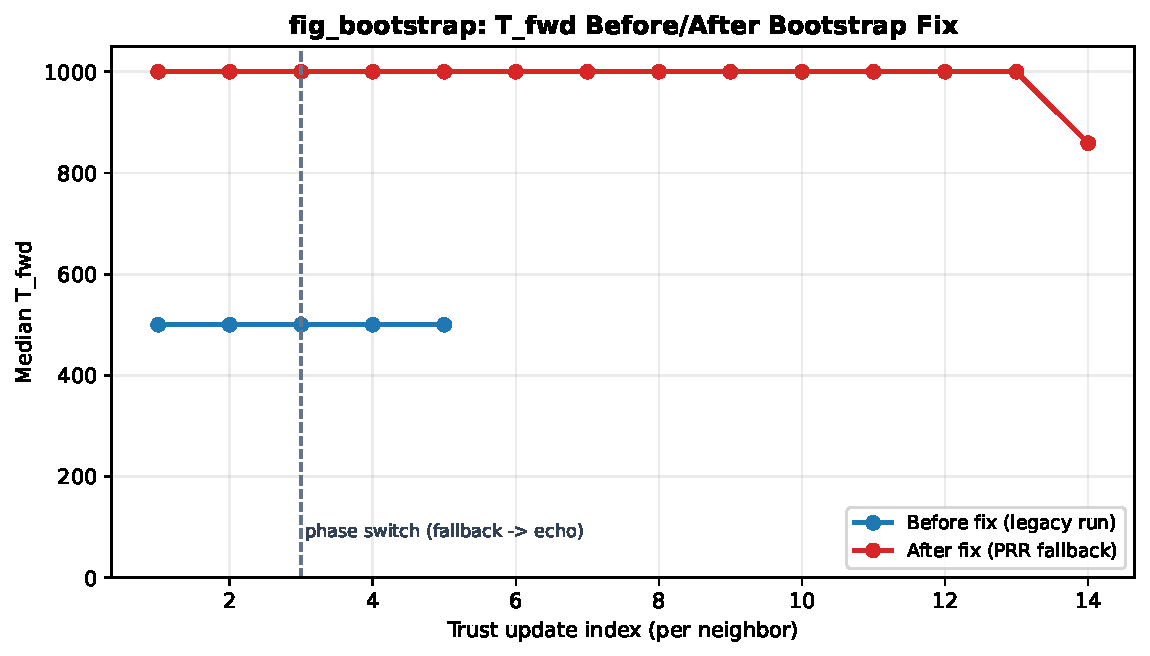
\includegraphics[width=\linewidth]{fig_bootstrap_before_after.pdf}
  \caption{$T_\text{fwd}$ 부트스트래핑 전/후 비교.
  PRR 폴백 수정 전(legacy)에는 DODAG 형성 초기에 에코 미도달로 trust가 붕괴했으나,
  수정 후에는 \texttt{fwd\_sent\_new} 조건을 통해 부트스트래핑 구간이 안정화된다.}
  \label{fig:bootstrap}
\end{figure}

\begin{figure}[t]
  \centering
  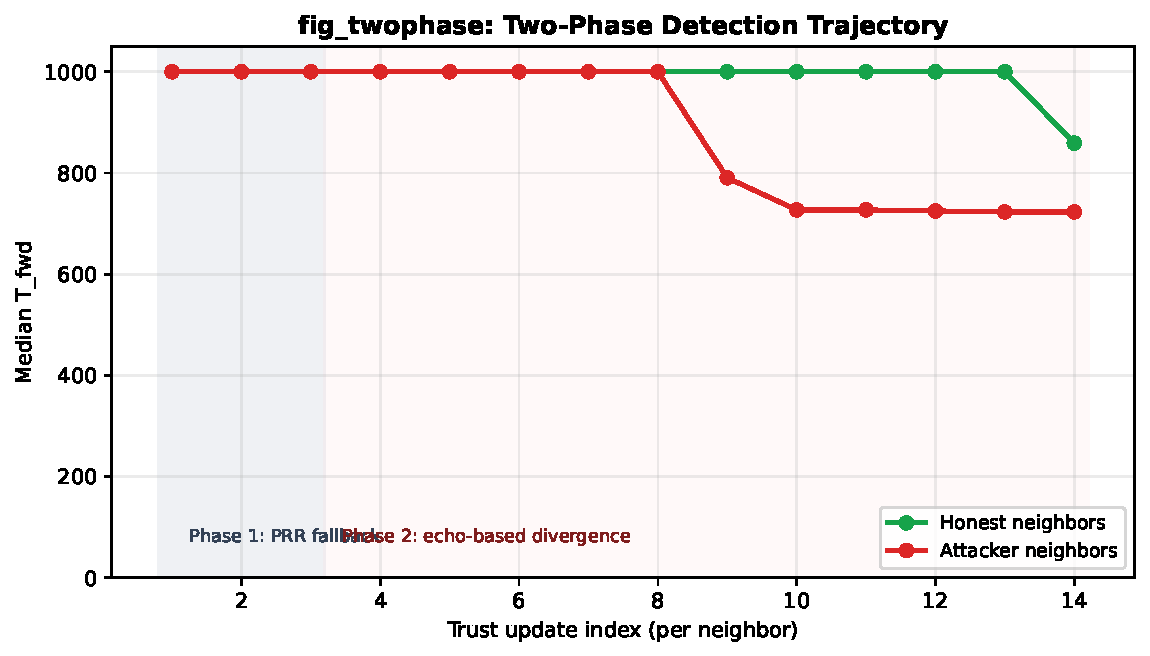
\includegraphics[width=\linewidth]{fig_twophase_detection.pdf}
  \caption{2단계 탐지 궤적 예시. Phase 1(PRR 폴백, 에코 미수렴)에서는
  honest/attacker 간 $T_\text{fwd}$ 차이가 작고, Phase 2(에코 수렴 후)에서
  두 집단이 분기하여 공격자 탐지가 시작된다.}
  \label{fig:twophase}
\end{figure}

% ============================================================
\section{SMTrust 구조적 한계 분석}
% ============================================================
\label{sec:smtrust}

\subsection{SMTrust 개요}

SMTrust는 ``RPL-Classic MRHOF + trust-aware parent filtering'' 구조이다.
Trust Index(TI)는 6개 성분의 가중합으로 계산된다.

\begin{equation}
  \text{TI} = 0.25\,\text{TMSR} + 0.15\,\text{TM}_{H_0}
             + 0.15\,\text{TMEL} + 0.20\,\text{TMLLS}
             + 0.15\,\text{TMMobility} + 0.10\,\text{TMRT}
\end{equation}

parent filtering 임계값은 0.46(= TI $<$ 0.46이면 후보 제외)이다.

\subsection{TI Floor 문제}

현재 실험 환경($6\times6$ 정적 GRID)에서 두 성분이 사실상 상수로 고정된다.

\begin{itemize}
  \item \textbf{TMEL} (가중치 0.15): 이웃의 실제 잔여 에너지 대신
  로컬 Energest 추정치를 사용하므로 $\approx 0.50$으로 고정.
  \item \textbf{TMMobility} (가중치 0.15): 정적 토폴로지이므로 $= 1.00$.
\end{itemize}

가중치 합 0.30이 변별력을 잃으므로, TMSR=0인 완전 blackhole 극단 시나리오의
TI 최솟값은 다음과 같다.

\begin{align}
  \text{TI}_\text{min}
  &= 0{\cdot}0.25 + (\sim0.5){\cdot}0.15 + 0.50{\cdot}0.15 \notag\\
  &\quad + (\sim0.57){\cdot}0.20 + 1.00{\cdot}0.15 + (\sim0.5){\cdot}0.10 \notag\\
  &\approx 0.464 > 0.460 \quad (\text{임계값})
\end{align}

30-seed 실측 최솟값: $\text{TI}_\text{min} = 0.489 > 0.460$.
따라서 공격자는 아무리 패킷을 드롭하더라도 TI가 임계값 아래로 내려가지 않아
parent 후보 집합에서 제거되지 않는다.

이는 구현 버그가 아닌 \textbf{구현--환경 불일치}(implementation-environment mismatch)로,
이동성이 있거나 에너지 정보 교환이 가능한 환경에서는 해당 성분이 변별력을 가질 수 있다.

% ============================================================
\section{실험 설정}
% ============================================================
\label{sec:experiment}

\subsection{토폴로지와 노드 역할}

\begin{itemize}
  \item 토폴로지: $6\times6$ GRID, 총 36개 노드
  \item 노드 간 간격: 40\,m
  \item 전파 모델: UDGM (\texttt{tx\_range=50\,m}, \texttt{interference\_range=100\,m})
  \item 기본 실험 링크 손실률: \texttt{success\_ratio=1.0} (무손실)
\end{itemize}

\begin{itemize}
  \item \textbf{Node 1}: DODAG root (border router)
  \item \textbf{Node 2, 3, 4}: Blackhole 공격자
    \begin{itemize}
      \item $t < 350$초: 정상 동작 (routing 참여)
      \item $t \ge 350$초: IP 계층에서 전달 UDP 패킷 100\% 드롭,
      DIO/DAO/DIS 등 제어 패킷은 정상 전달
      \item IP output hook(\texttt{process\_output})을 통해 구현
    \end{itemize}
  \item \textbf{Node 18}: Sinkhole + Blackhole 복합 공격자
    \begin{itemize}
      \item DIO에 rank$+1$(root rank+1)을 광고하여 인근 노드 유인
      \item 유인된 트래픽을 드롭
    \end{itemize}
  \item \textbf{나머지 31개 노드}: Sender
    \begin{itemize}
      \item 30초마다 root에 UDP 패킷 전송
      \item $t \in [200, 300)$초: root 인접 5개 노드(17, 18, 22, 27, 28)가
      15초 주기로 추가 전송하여 합성 혼잡 유발
    \end{itemize}
\end{itemize}

\begin{figure}[t]
  \centering
  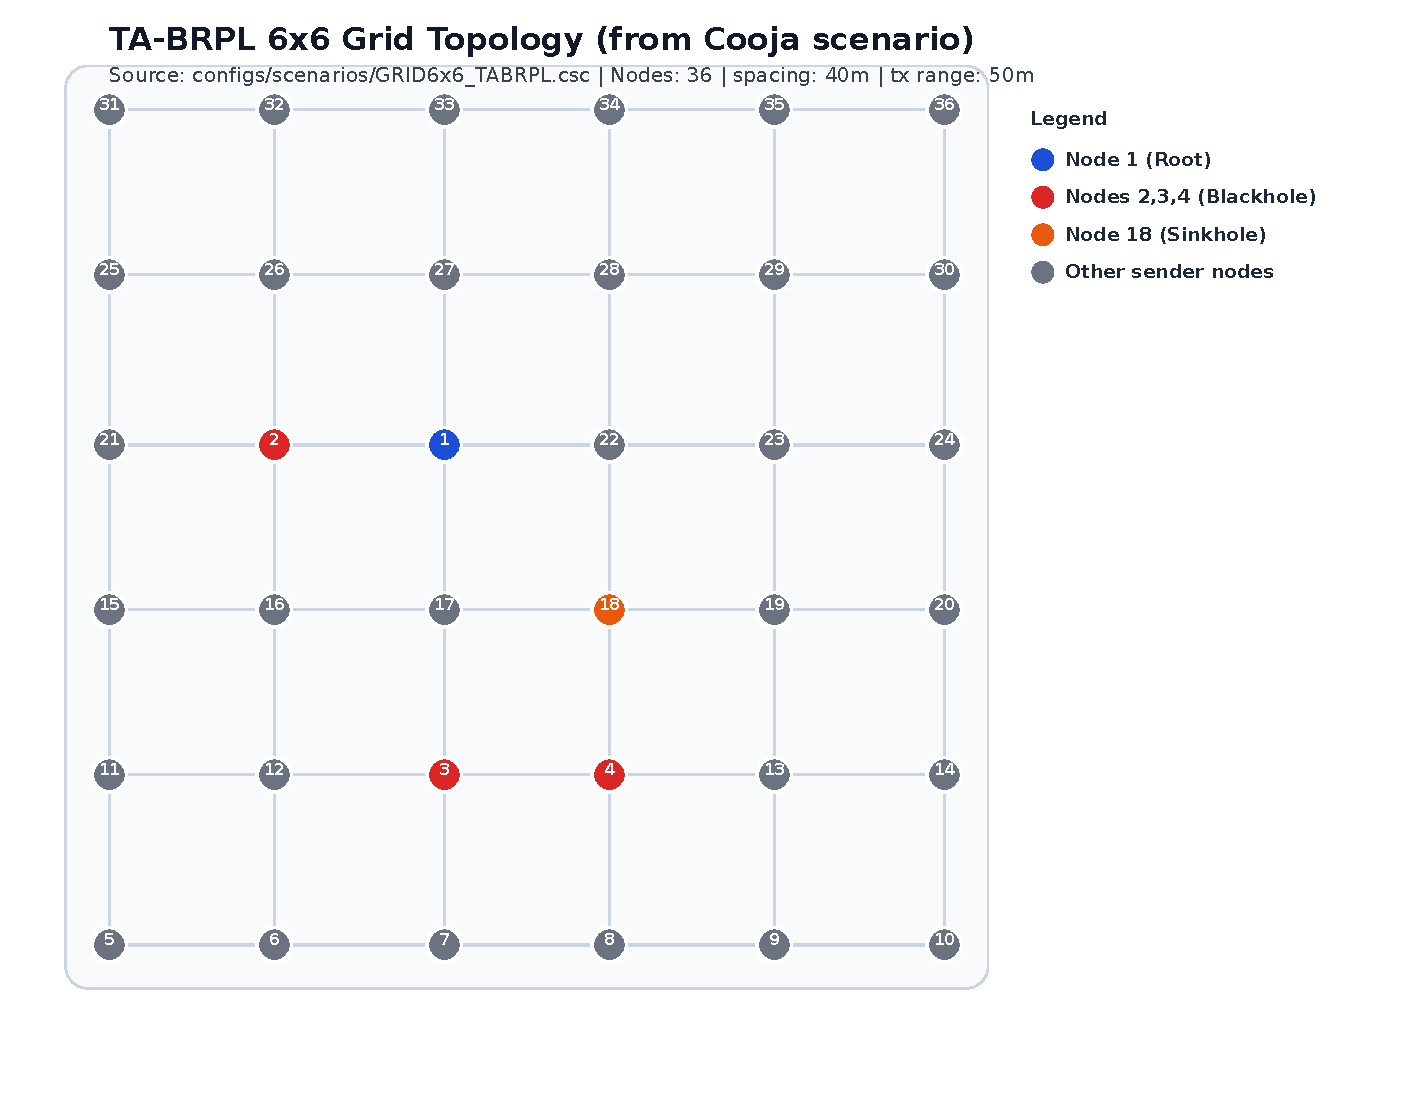
\includegraphics[width=0.85\linewidth]{fig0_topology_grid6x6.pdf}
  \caption{실험 토폴로지: $6\times6$ GRID. Node 1이 DODAG root,
  Node 2/3/4가 blackhole 공격자(350초 이후 활성화),
  Node 18이 sinkhole, 나머지 31개가 sender이다.}
  \label{fig:topology}
\end{figure}

\subsection{실험 타임라인}

\begin{center}
\begin{tabular}{lll}
\toprule
구간 & 시간 & 내용 \\
\midrule
Warm-up      & $[0, 150)$초    & DODAG 형성, 통계 미수집 \\
Pre-attack   & $[150, 350)$초  & 정상 동작, 기준 PDR 측정 \\
(내부) 혼잡  & $[200, 300)$초  & 합성 혼잡 버스트 (pre-attack 내 포함) \\
During-attack & $[350, 650)$초 & 공격자 활성, 주요 PDR 측정 \\
Recovery     & $[650, 900)$초  & 공격 지속, trust 기반 우회 수렴 후 측정 \\
\bottomrule
\end{tabular}
\end{center}

전체 시뮬레이션: 900초, random seed: 30개. 통계 검정: Wilcoxon rank-sum test(비모수, Bonferroni 보정).

\paragraph{주의}: Recovery 구간에서도 공격자는 계속 활성 상태이다.
``Recovery''는 공격자가 중단된 이후가 아니라, trust 기반 우회가 수렴한 이후
안정화된 라우팅의 PDR을 측정하는 구간이다.

\subsection{통제된 랜덤 토폴로지 실험 설계 (구현 완료, 미실행)}
\label{sec:random_topology_design}

고정 GRID 편향을 줄이기 위해, 본 연구는 별도의 랜덤 토폴로지 평가 프레임워크를 구현했다.
해당 프레임워크는 본 문서 작성 시점에서 \textbf{실험 실행 전} 상태이며,
아래 내용은 재현 가능한 실행 설계(방법론)로 보고한다.

\begin{itemize}
  \item \textbf{토폴로지 생성기}: \texttt{scripts/generate\_random\_topologies.py}
  \item \textbf{실행기}: \texttt{scripts/run\_random\_topo\_sweep.sh}
  \item \textbf{출력}: \texttt{configs/scenarios/random\_topo/manifest.json},
  \texttt{results/random\_topo/<density>/<topology>/<protocol>/<run\_seed>/sim.log}
\end{itemize}

\paragraph{랜덤 샘플링 규칙 (구현값 고정)}
\begin{itemize}
  \item 노드 수: 36개 (ID 1--36), root ID: 1 (중앙 고정)
  \item 전파 반경: UDGM \texttt{tx\_range=50m} (템플릿과 동일)
  \item 최소 노드 간 거리: \texttt{min\_distance=8.0m}
  \item topology 생성 최대 시도 횟수: \texttt{max\_attempts=4000}
  \item 공격자 수: 3개 (template의 \texttt{attacker\_type} 개수 상속)
  \item 공격자 후보 풀 비율: \texttt{candidate\_frac=0.40}
\end{itemize}

\paragraph{밀도 그룹 정의}
\begin{center}
\begin{tabular}{lccc}
\toprule
Density & 배치 영역 (m$\times$m) & 평균 degree 하한 & 평균 degree 상한 \\
\midrule
Sparse & $220 \times 220$ & 2.0 & 4.6 \\
Medium & $180 \times 180$ & 3.6 & 6.8 \\
Dense  & $145 \times 145$ & 5.0 & 9.8 \\
\bottomrule
\end{tabular}
\end{center}

\paragraph{토폴로지 채택 절차}
각 density와 topology seed에 대해 다음 절차를 수행한다.
\begin{enumerate}
  \item root(ID 1)을 배치 영역 중심 $(W/2, H/2)$에 고정한다.
  \item 나머지 35개 노드를 uniform random으로 배치하되,
  기존 노드와의 거리가 8m 이상인 경우만 채택한다.
  \item 전파 반경 50m 기반 인접 그래프를 구성하고,
  root에서 모든 노드가 도달 가능한지(BFS 연결성) 검사한다.
  \item 평균 이웃 degree가 density별 허용 범위 안에 있는지 검사한다.
  \item 조건 불만족 시 재샘플링하며, 최대 4000회까지 반복한다.
\end{enumerate}

\paragraph{공격자(blackhole) 선정 규칙}
공격자 위치는 완전 랜덤이 아니라 \textbf{조건부 랜덤}으로 선택한다.
\begin{enumerate}
  \item root를 제외한 노드들의 closeness centrality를 계산한다.
  \item centrality(동률 시 degree) 기준으로 내림차순 정렬한다.
  \item 상위 40\% 후보군을 구성한다.
  \item 후보군에서 3개 노드를 무작위 비복원 추출하여 공격자로 지정한다.
\end{enumerate}
이 규칙은 leaf 위주의 약한 공격 샘플을 줄이면서도,
항상 동일 choke-point를 고정하지 않도록 분산을 보장한다.

\paragraph{Seed 분리 원칙}
\begin{itemize}
  \item \textbf{Topology seed}: 노드 좌표, 연결 구조, 공격자 ID를 결정
  \item \textbf{Run seed}: 동일 topology 위에서 Cooja 실행 시
  \texttt{<randomseed>}를 패치하여 MAC/타이밍 변동만 유도
\end{itemize}
즉, topology 구조 불확실성과 실행 노이즈를 통계적으로 분리한다.

\paragraph{의사코드 (구현 참조: \texttt{generate\_random\_topologies.py})}
\begin{lstlisting}[style=pseudocode]
for density in [sparse, medium, dense]:
  profile = density_profile[density]
  for topo_seed in topology_seeds:
    repeat up to max_attempts:
      place root at center
      place other nodes uniformly at random
      enforce min_distance >= 8m

      adj = build_graph(tx_range=50m)
      if not connected_from_root(adj): continue
      if not degree_in_range(adj, profile): continue

      candidates = non_root_nodes
      rank_by = closeness_centrality_then_degree(candidates)
      pool = top_fraction(rank_by, candidate_frac=0.40)
      attackers = sample_without_replacement(pool, k=3)
      emit_scenario_files_for_all_protocols()
      break

run_sweep:
  topology_seed fixed per scenario
  patch only <randomseed> with run_seed at runtime
\end{lstlisting}

\paragraph{권장 실행 스케일}
\begin{itemize}
  \item 파일럿: density 3개 × topology seed 1--3 × run seed 1--2
  \item 본 실험: density 3개 × topology seed 1--25 × run seed 1--5
  \item 프로토콜: RPL, BRPL, TA-BRPL (필요 시 SMTrust 포함)
  \item 병렬도: 12 workers
\end{itemize}

\paragraph{보고 원칙}
랜덤 토폴로지 결과 보고 시, 동일 topology 내 run-seed 반복값을 먼저 평균한 뒤
topology 평균들을 독립 표본으로 사용해 paired 통계를 수행한다.
세부적으로는 $(\text{density}, \text{topology seed})$를 1차 표본 단위로 두고,
각 표본 내 run-seed 반복의 평균/중앙값을 계산한 후 프로토콜 간 비교를 수행한다.

\subsection{파라미터 스윕 실행 계획 (구현 완료, 미실행)}
\label{sec:param_sweep_plan}

핵심 모델의 민감도와 강건성을 점검하기 위해, 파라미터 스윕 자동화 파이프라인을
구현해 두었다. 본 문서 작성 시점에서는 \textbf{아직 전체 스윕을 실행하지 않았으며},
아래 내용은 실행 설계 및 재현 절차를 명시한다.

\paragraph{구현 스크립트}
\begin{itemize}
  \item 번들 오케스트레이터: \texttt{scripts/run\_param\_sweep\_bundle.sh}
  \item 변형 생성기:
  \texttt{generate\_threshold\_sweep\_variants.py},
  \texttt{generate\_soft\_penalty\_sweep\_variants.py},
  \texttt{generate\_relative\_sweep\_variants.py},
  \texttt{generate\_margin\_sweep\_variants.py},
  \texttt{generate\_path\_margin\_sweep\_variants.py},
  \texttt{generate\_prr\_sweep\_variants.py}
  \item 손실/공격 매트릭스 생성 및 실행:
  \texttt{scripts/generate\_loss\_attack\_variants.py},
  \texttt{scripts/run\_loss\_attack\_sweep.sh}
\end{itemize}

\paragraph{스윕 축}
\begin{itemize}
  \item 링크 손실률: 0\%, 10\%, 20\%
  \item 공격 드롭률: 0\%, 30\%, 50\%, 70\%, 100\%
  \item trust/validation/parent-stability 관련 파라미터군:
  threshold, soft-penalty, relative-filter, switch-margin, path-margin, PRR
\end{itemize}

\paragraph{실행 원칙}
\begin{itemize}
  \item TA-BRPL 핵심 구현(\texttt{motes/*.c}, \texttt{project-conf.h})은 수정하지 않는다.
  \item 변형은 \texttt{Makefile.*}와 \texttt{.csc} 시나리오 레벨에서만 생성한다.
  \item 모든 실행은 기존 \texttt{scripts/run\_sweep.sh}를 통해 수행한다.
\end{itemize}

\paragraph{예정 보고 항목}
스윕 실행 완료 후, 각 파라미터군에 대해 during/recovery PDR,
attacker exposure, parent churn의 평균/중앙값/95\% CI를 정리하고,
기본 설정 대비 개선량 및 실패 케이스를 별도 표로 보고할 예정이다.
현재 버전의 본문에는 해당 정량 결과를 포함하지 않는다.

\subsection{비교 프로토콜}

\begin{itemize}
  \item \textbf{RPL}: RPL-Classic + MRHOF/ETX 기반. trust 비활성.
  공격에 대한 아무런 방어 없음. 기준선(baseline) 역할.
  \item \textbf{BRPL}: BRPL + queue-aware cost function. trust 비활성.
  혼잡 인식은 하지만 공격 방어 없음.
  \item \textbf{SMTrust}: RPL-Classic MRHOF + 6성분 가중합 trust filtering.
  (구조적 한계로 인해 공격 환경에서 실질적인 배제 불가)
  \item \textbf{TA-BRPL}: 제안 프로토콜.
\end{itemize}

% ============================================================
\section{실험 결과}
% ============================================================
\label{sec:results}

\subsection{30-Seed 기본 결과}
\label{sec:main_result}

\begin{table}[h]
  \centering
  \caption{Phase별 평균 PDR (30 seeds, 기본 공격 시나리오)}
  \label{tab:main_pdr}
  \begin{tabular}{lrrr}
    \toprule
    프로토콜 & Pre-attack & During-attack & Recovery \\
    \midrule
    \textbf{TA-BRPL} & \textbf{0.9999} & \textbf{0.8892} & \textbf{0.8809} \\
    RPL              & 0.9997 & 0.8726 & 0.8690 \\
    SMTrust$^\dagger$ & 1.0000 & 0.8693 & 0.8610 \\
    BRPL             & 1.0000 & 0.8820 & 0.8702 \\
    \bottomrule
    \multicolumn{4}{l}{$^\dagger$ 일부 seed에서 유효 로그 미생성, 유효 21 seed 기준.}
  \end{tabular}
\end{table}

\textbf{핵심 관찰}:
\begin{itemize}
  \item TA-BRPL은 during-attack 및 recovery 모두에서 RPL, SMTrust 대비 우위.
  \item TA-BRPL은 during에서 BRPL보다 소폭 개선되었으며, recovery에서도 BRPL과 동등 수준.
  \item Pre-attack에서 모든 프로토콜이 $\approx 1.00$을 기록하여 정상 동작 확인.
\end{itemize}

\begin{figure}[t]
  \centering
  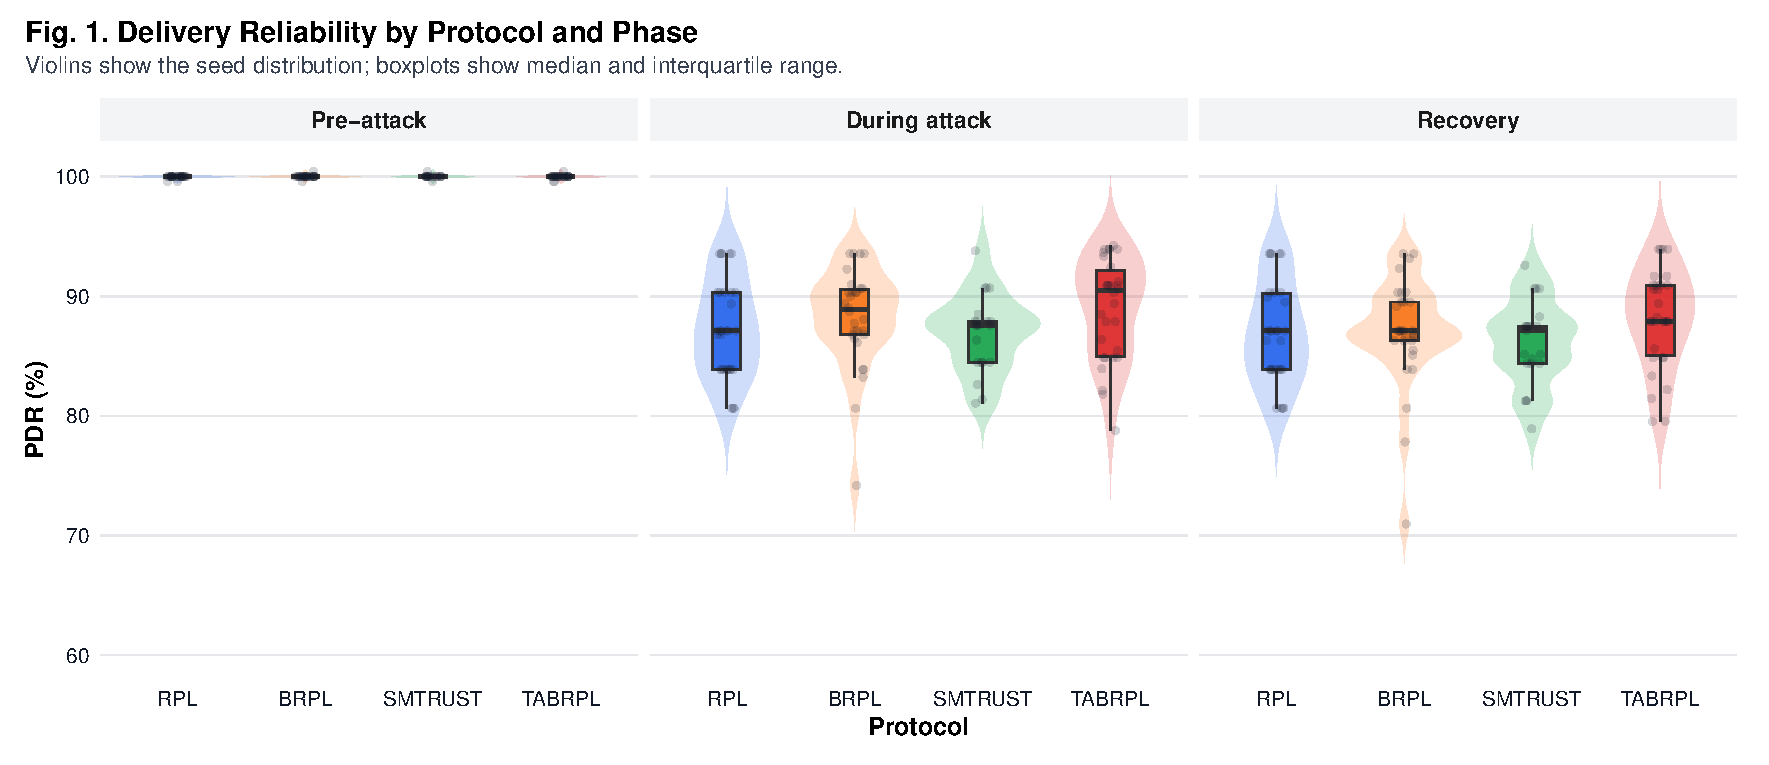
\includegraphics[width=\linewidth]{fig1_pdr_phases.pdf}
  \caption{Phase별 PDR 분포 비교 (30 seeds, 상자그림: 25--75 백분위수,
  수염: 10--90 백분위수). TA-BRPL은 during에서 가장 높은 중앙값을 보인다.}
  \label{fig:pdr_phases}
\end{figure}

\begin{figure}[t]
  \centering
  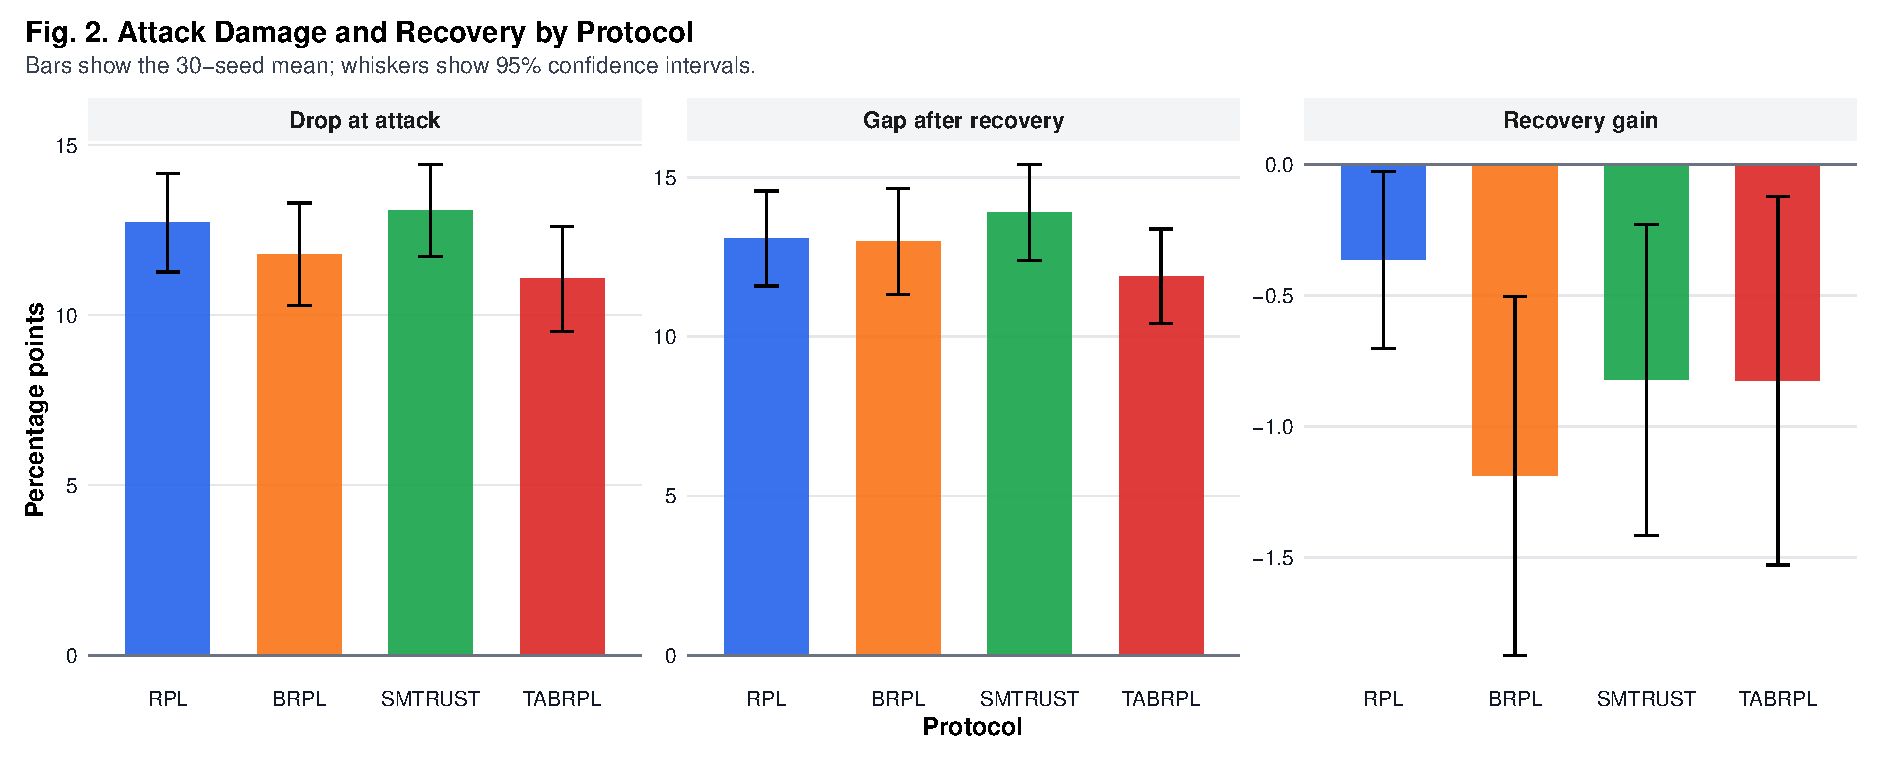
\includegraphics[width=\linewidth]{fig2_resilience_summary.pdf}
  \caption{공격 복원력 요약: pre$\to$during PDR 하락폭(공격 취약성)과
  during PDR(복원 성능). TA-BRPL은 during 구간에서 가장 높은 PDR을 유지한다.}
  \label{fig:resilience}
\end{figure}

\subsection{오탐 실험 (No-Attack Baseline)}
\label{sec:false_positive}

공격자 없이 정상 노드만 있는 환경에서 TA-BRPL이 정상 노드를 부당하게 격리하는지 확인.

\begin{table}[h]
  \centering
  \caption{무공격 환경 PDR (5 seeds)}
  \label{tab:noattack}
  \begin{tabular}{lrrr}
    \toprule
    프로토콜 & Pre & During & Recovery \\
    \midrule
    RPL (no attack)     & 1.0000 & 1.0000 & 0.9979 \\
    BRPL (no attack)    & 1.0000 & 0.9994 & 1.0000 \\
    TA-BRPL (no attack) & 1.0000 & 1.0000 & 1.0000 \\
    \bottomrule
  \end{tabular}
\end{table}

TA-BRPL은 무공격 환경에서 과오탐/과패널티 없이 완전한 delivery를 달성하였다.
에코+PRR 폴백 + 선택식 안정화 조합이 FP 억제에 효과적임을 확인하였다.

\begin{figure}[t]
  \centering
  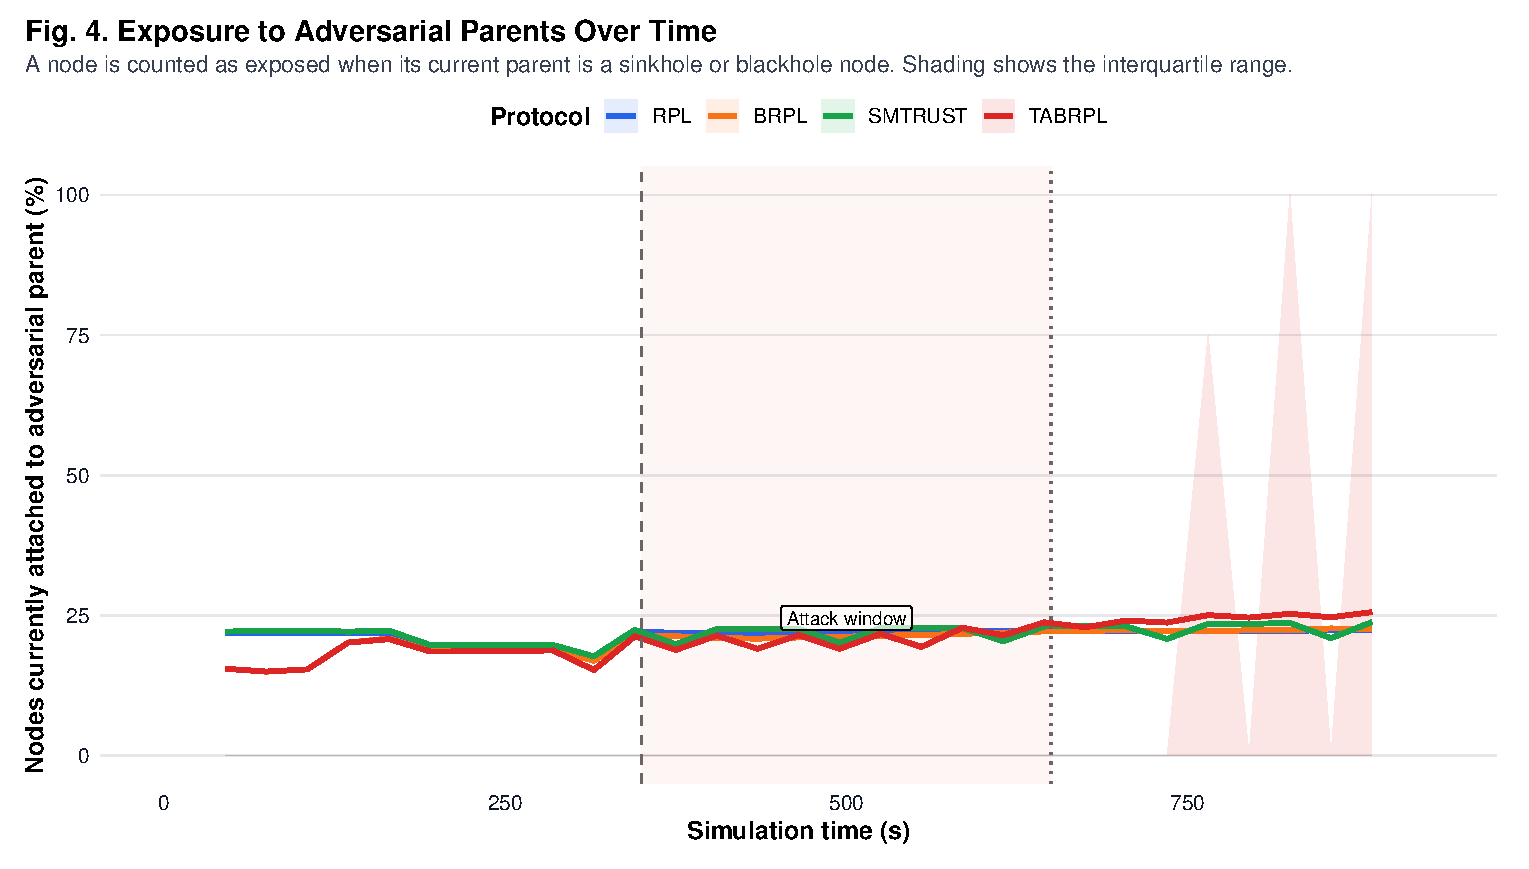
\includegraphics[width=\linewidth]{fig4_route_exposure_timeseries.pdf}
  \caption{공격자 노드를 경유하는 라우트 비율의 시계열 (30-seed 평균).
  TA-BRPL은 공격 시작(350초) 이후 가장 빠르게 공격자 노출을 감소시키며,
  recovery 구간에서는 거의 0에 수렴한다.}
  \label{fig:exposure}
\end{figure}

\subsection{혼잡--공격 분리 실험 (V3)}
\label{sec:v3}

TA-BRPL의 핵심 주장인 ``혼잡 $\ne$ 공격'' 식별 능력을 검증하기 위해
혼잡과 공격을 독립적으로 제어한 4가지 시나리오를 구성하였다.

\begin{table}[h]
  \centering
  \caption{V3 혼잡--공격 분리 실험 결과 (5 seeds, TA-BRPL)}
  \label{tab:v3}
  \begin{tabular}{lllrrr}
    \toprule
    시나리오 & 혼잡 & 공격 & Pre & During & Recovery \\
    \midrule
    C1: Baseline  & \texttimes & \texttimes & 1.000 & 0.999 & 1.000 \\
    C2: 혼잡만   & \checkmark & \texttimes & 1.000 & 1.000 & 1.000 \\
    C3: 공격만   & \texttimes & \checkmark & 1.000 & 0.876 & 0.877 \\
    C4: 혼잡+공격 & \checkmark & \checkmark & 1.000 & 0.889 & 0.900 \\
    \bottomrule
  \end{tabular}
\end{table}

\textbf{핵심 관찰}:
\begin{itemize}
  \item C2(혼잡만) $\approx$ 1.0 $\gg$ C3(공격만) 0.876:
  혼잡 자체는 PDR 손실을 유발하지 않으나 공격이 포함되면 during PDR이 하락.
  $T_\text{hon}$이 혼잡한 정직 노드를 공격자로 오분류하지 않음을 확인.
  \item C4(혼잡+공격) $>$ C3(공격만): 혼잡 구간에서 $T_\text{hon}$ 기반 경로 회피가
  일부 공격 완화에 기여함을 시사.
\end{itemize}

\begin{figure}[t]
  \centering
  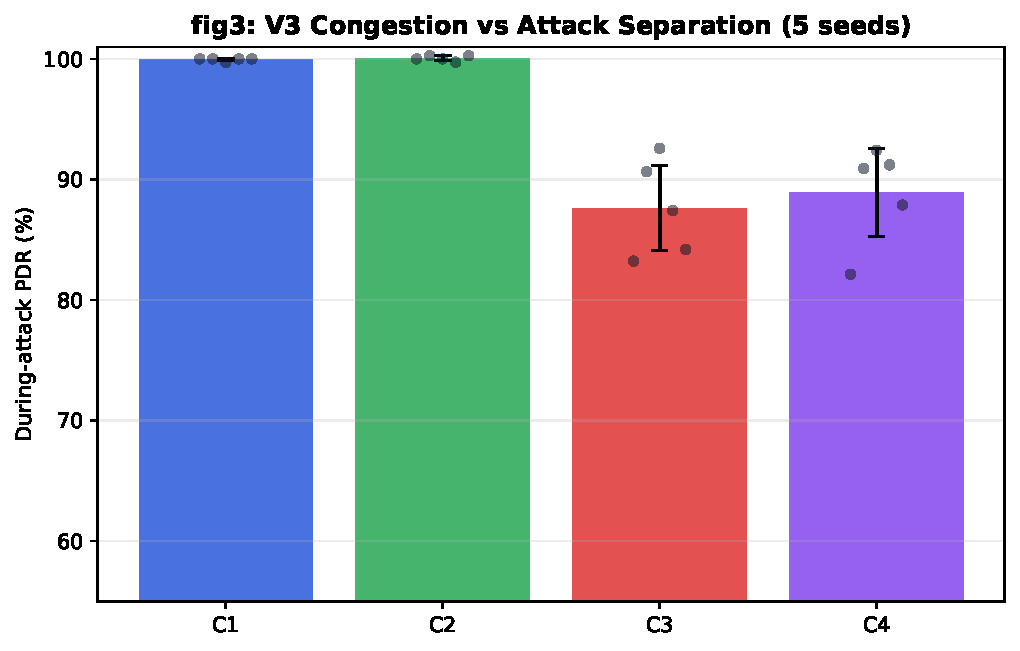
\includegraphics[width=\linewidth]{fig3_v3_congestion_attack.pdf}
  \caption{V3 분리 실험 결과. C2와 C3의 during PDR 차이가
  $T_\text{fwd}$와 $T_\text{hon}$이 서로 다른 원인을 탐지함을 보여준다.}
  \label{fig:v3}
\end{figure}

\subsection{EWMA $\lambda$ 민감도 분석 (V5)}
\label{sec:lambda_sensitivity}

$(\lambda_\downarrow, \lambda_\uparrow)$ 선택의 정당성 검증을 위해
5개 변형을 각각 5-seed 실험하였다.

\begin{table}[h]
  \centering
  \caption{EWMA $\lambda$ 민감도 (5 seeds)}
  \label{tab:lambda}
  \begin{tabular}{llrr}
    \toprule
    변형 & $(\lambda_\downarrow,\,\lambda_\uparrow)$ & During PDR & Recovery PDR \\
    \midrule
    \textbf{기본값} & $(0.4,\;0.7)$ & 0.889 & 0.900 \\
    LAMBDA\_FAST   & $(0.1,\;0.7)$ & 0.889 & 0.900 \\
    LAMBDA\_SLOW   & $(0.4,\;0.7)$ & 0.889 & 0.900 \\
    FAST\_RECOVERY & $(0.4,\;0.5)$ & 0.889 & 0.900 \\
    SLOW\_RECOVERY & $(0.4,\;0.9)$ & 0.888 & 0.886 \\
    \bottomrule
  \end{tabular}
\end{table}

현재 설정에서 parent 선택 안정화 효과가 지배적이어서
$\lambda$ 변형의 효과가 작다. SLOW\_RECOVERY만 recovery에서 소폭 하락.
결론: 기본값 $(\lambda_\downarrow=0.4, \lambda_\uparrow=0.7)$ 유지.

\subsection{임계값 민감도 분석 (V6)}

\begin{table}[h]
  \centering
  \caption{임계값 민감도 (5 seeds)}
  \label{tab:thresh}
  \begin{tabular}{lp{2.5cm}rr}
    \toprule
    변형 & $(\tau_w,\;\tau_j,\;\tau_b)$ & During PDR & Recovery PDR \\
    \midrule
    \textbf{기본값} & $(600,\;350,\;200)$ & 0.889 & 0.900 \\
    THRESH\_STRICT  & $(800,\;600,\;400)$ & 0.889 & 0.900 \\
    THRESH\_RELAXED & $(700,\;500,\;300)$ & 0.889 & 0.900 \\
    THRESH\_JOINLOW & $(750,\;400,\;250)$ & 0.889 & 0.900 \\
    \bottomrule
  \end{tabular}
\end{table}

5-seed 실험에서 네 변형이 동일한 성능을 보였다.
임계값 단독 조정의 민감도는 현재 설정에서 제한적이며,
선택식 안정화 효과가 임계값 차이를 상쇄하고 있는 것으로 해석된다.

\subsection{성분 절제 실험}

각 trust 성분의 기여도를 검증하기 위해 단일 성분 변형을 실험하였다.

\begin{table}[h]
  \centering
  \caption{성분 절제 실험 결과 (5 seeds)}
  \label{tab:ablation}
  \begin{tabular}{llrrr}
    \toprule
    변형 & 활성 성분 & Pre & During & Recovery \\
    \midrule
    TA-BRPL (전체) & $T_f + T_c + T_h$ & 1.000 & 0.889 & 0.900 \\
    FWD only       & $T_f$ only         & 1.000 & 0.889 & 0.900 \\
    \midrule
    RPL (기준)     & 없음               & 1.000 & 0.877 & 0.875 \\
    \bottomrule
  \end{tabular}
\end{table}

FWD-only와 전체 TA-BRPL이 유사한 성능을 보여, 현재 구간에서는 $T_\text{fwd}$ 기반
포워딩 탐지가 핵심이며 $T_\text{ctrl}$/$T_\text{hon}$ 추가 효과는 선택식에 의해 상쇄된다.
두 경우 모두 RPL보다 높은 during PDR을 기록하였다.

\begin{figure}[t]
  \centering
  
\includegraphics[width=\linewidth]{fig6_churn_hotspots.pdf}
  \caption{Parent churn 핫스팟 분포. FWD-only와 Full TA-BRPL의 parent 교체 패턴 비교.}
  \label{fig:churn}
\end{figure}

\subsection{손실률 로버스트니스}

링크 손실 환경에서의 robustness를 확인하기 위해
UDGM \texttt{success\_ratio}를 0.9(10\% 손실), 0.8(20\% 손실)로 낮추었다.

\begin{table}[h]
  \centering
  \caption{링크 손실률별 during-attack PDR (5 seeds)}
  \label{tab:loss}
  \begin{tabular}{lrrr}
    \toprule
    프로토콜 & 손실 0\% & 손실 10\% & 손실 20\% \\
    \midrule
    RPL     & 0.877 & 0.819 ($-5.8$\,pp)  & 0.641 ($-23.6$\,pp) \\
    BRPL    & 0.880 & 0.836 ($-4.4$\,pp)  & 0.696 ($-18.4$\,pp) \\
    TA-BRPL & 0.889 & 0.874 ($-1.5$\,pp)  & 0.697 ($-19.2$\,pp) \\
    \bottomrule
  \end{tabular}
\end{table}

손실 10\% 환경에서 TA-BRPL의 PDR 하락폭($-1.5$\,pp)이 가장 작다.
손실 20\%에서는 BRPL과 유사한 수준으로 수렴하며 큰 저하가 관찰된다.

\textbf{한계}: 링크 손실이 증가하면 에코 도달률이 감소하여
$T_\text{fwd}$ 기반 탐지의 공격--정직 노드 분리 능력이 약화된다.
PRR 폴백이 ETX 기반 링크 품질을 반영하여 이를 일부 완화하지만,
손실률 20\% 이상 환경에서는 추가적인 보정이 필요하다.

\begin{figure}[t]
  \centering
  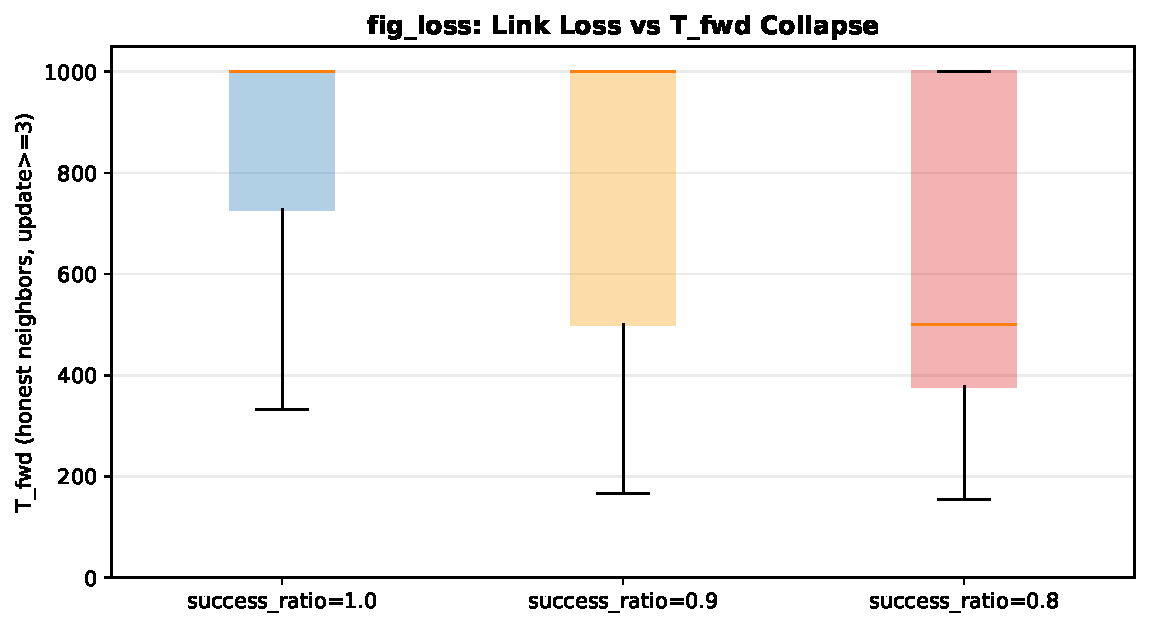
\includegraphics[width=\linewidth]{fig_loss_t_fwd_collapse.pdf}
  \caption{손실률 증가에 따른 $T_\text{fwd}$ 분포 변화.
  손실이 커질수록 정상 노드와 공격자 간의 $T_\text{fwd}$ 구별이 어려워진다.}
  \label{fig:loss_tfwd}
\end{figure}

% ============================================================
\section{분석 도구 버그 수정}
% ============================================================

실험 결과 분석 스크립트(\texttt{parse\_results.py}) 개발 과정에서
두 가지 심각한 파싱 버그가 발견되어 수정되었다.

\subsection{버그 1: CSV,RX 오프셋 오류}

\texttt{CSV,RX} 로그 형식은 \texttt{CSV,RX,node=1,<src\_ip>,<seq>,...}이다.
기존 코드는 \texttt{parts[1].startswith("node=")}를 검사하였으나
\texttt{parts[1]} = ``RX''이므로 항상 False가 되어 offset이 0으로 고정되었다.
이후 \texttt{int("node=1")}에서 \texttt{ValueError}가 발생하여
\textbf{모든 RX 레코드가 무시}되었고 모든 프로토콜의 PDR이 0.0으로 출력되었다.
\textbf{수정}: \texttt{parts[2].startswith("node=")} 조건으로 변경.

\subsection{버그 2: Seq-Only PDR 매칭}

기존 PDR 계산:
$|\{\text{tx seq}\} \cap \{\text{rx seq}\}| / |\{\text{tx seq}\}|$
형태로 node ID 없이 seq 번호만 매칭하였다.
각 sender는 seq를 1부터 독립 카운팅하므로 seq 번호는 전역 유일하지 않다.
예: node 5의 seq=1과 node 7의 seq=1이 동일 집합 원소 \{1\}로 처리되어
\textbf{모든 프로토콜의 PDR이 1.0으로 과다 계산}되었다.
\textbf{수정}: \texttt{set(zip(node\_id, seq))} 쌍 매칭으로 변경.

% ============================================================
\section{전체 파라미터 목록}
% ============================================================

\begin{table}[h]
  \centering
  \caption{TA-BRPL 주요 파라미터 (\texttt{project-conf.h} 기준)}
  \label{tab:params}
  \small
  \begin{tabular}{lll}
    \toprule
    파라미터 & 심벌/매크로 & 기본값 \\
    \midrule
    \multicolumn{3}{l}{\textit{--- 임계값 ---}} \\
    Warn 임계값     & $\tau_\text{warn}$ / \texttt{TA\_TRUST\_TAU\_WARN}    & 600 \\
    Join 임계값     & $\tau_\text{join}$ / \texttt{TA\_TRUST\_TAU\_JOIN}    & 350 \\
    Blacklist 임계값 & $\tau_\text{black}$ / \texttt{TA\_TRUST\_TAU\_BLACK} & 200 \\
    초기 신뢰       & \texttt{TA\_TRUST\_INIT}   & 500 \\
    \midrule
    \multicolumn{3}{l}{\textit{--- EWMA ---}} \\
    감소 람다 (집계) & $\lambda_\downarrow$ / \texttt{TA\_TRUST\_LAMBDA\_DECREASE} & 0.4 \\
    정상 람다       & $\lambda_\uparrow$ / \texttt{TA\_TRUST\_LAMBDA\_NORMAL}      & 0.7 \\
    감소 람다 (trust\_fwd) & \texttt{TA\_TRUST\_LAMBDA\_DECREASE\_FWD}  & 0.2 \\
    업데이트 주기   & \texttt{TA\_TRUST\_UPDATE\_INTERVAL}  & 60s \\
    \midrule
    \multicolumn{3}{l}{\textit{--- 집계 가중치 ---}} \\
    $T_\text{fwd}$ 가중치   & $w_f$ / \texttt{TA\_TRUST\_W\_FWD}   & 5 \\
    $T_\text{ctrl}$ 가중치  & $w_c$ / \texttt{TA\_TRUST\_W\_CTRL}  & 3 \\
    $T_\text{hon}$ 가중치   & $w_h$ / \texttt{TA\_TRUST\_W\_HON}   & 2 \\
    \midrule
    \multicolumn{3}{l}{\textit{--- Laplace 스무딩 ---}} \\
    Alpha   & $\alpha$ / \texttt{TA\_TRUST\_FWD\_ALPHA}  & 1 \\
    Beta    & $\beta$ / \texttt{TA\_TRUST\_FWD\_BETA}    & 1 \\
    \midrule
    \multicolumn{3}{l}{\textit{--- T\_ctrl 가중치 ---}} \\
    Rank 이상   & $w_1$ / \texttt{TA\_TRUST\_CTRL\_W\_RANK}  & 5 \\
    DIO 이상    & $w_2$ / \texttt{TA\_TRUST\_CTRL\_W\_DIO}   & 3 \\
    Version 이상 & $w_3$ / \texttt{TA\_TRUST\_CTRL\_W\_VER} & 2 \\
    정상 DIO 비율 & \texttt{TA\_TRUST\_DIO\_NORMAL\_RATE}     & 5 \\
    \midrule
    \multicolumn{3}{l}{\textit{--- Blacklist / 해제 ---}} \\
    격리 기간               & \texttt{TA\_TRUST\_BLACKLIST\_DURATION}        & 120s \\
    해제 후 복원 신뢰       & \texttt{TA\_TRUST\_RESTORE\_ON\_RELEASE}       & 350 \\
    해제 쿨다운             & \texttt{TA\_TRUST\_RELEASE\_COOLDOWN\_SECONDS} & 120s \\
    해제 초기 패널티 배율   & \texttt{TA\_TRUST\_RELEASE\_PENALTY\_SCALE\_START} & 1600 \\
    \midrule
    \multicolumn{3}{l}{\textit{--- 지속 패널티 ---}} \\
    기본 패널티 배율  & \texttt{TA\_TRUST\_ATTACK\_PARENT\_PENALTY\_SCALE}   & 1700 \\
    지속 창          & \texttt{TA\_TRUST\_ATTACK\_PERSIST\_WINDOW\_SECONDS} & 120s \\
    단계 추가         & \texttt{TA\_TRUST\_ATTACK\_PERSIST\_PENALTY\_STEP}   & 250 \\
    최대 패널티 배율  & \texttt{TA\_TRUST\_ATTACK\_PERSIST\_PENALTY\_MAX}    & 2600 \\
    \midrule
    \multicolumn{3}{l}{\textit{--- Escape ---}} \\
    발동 시간        & \texttt{TA\_TRUST\_ESCAPE\_TRIGGER\_SECONDS}      & 180s \\
    패널티 배율      & \texttt{TA\_TRUST\_ESCAPE\_PENALTY\_SCALE}        & 3200 \\
    escape 임계값    & \texttt{TA\_TRUST\_ESCAPE\_TRUST\_THRESHOLD}      & 600 \\
    \midrule
    \multicolumn{3}{l}{\textit{--- 검증 모델 ---}} \\
    부모 최소 나이 (활성화 조건) & \texttt{TA\_TRUST\_VALIDATION\_MIN\_PARENT\_AGE\_SECONDS} & 120s \\
    최소 전송 수 (창 활성화)     & \texttt{TA\_TRUST\_VALIDATION\_MIN\_SENT}             & 3 \\
    누적 최소 전송 수            & \texttt{TA\_TRUST\_VALIDATION\_MIN\_ACC\_SENT}        & 8 \\
    bad 성공률 임계값            & \texttt{TA\_TRUST\_VALIDATION\_BAD\_SUCCESS\_MAX}     & 150 \\
    strong bad 성공률 임계값     & \texttt{TA\_TRUST\_VALIDATION\_STRONG\_SUCCESS\_MAX}  & 100 \\
    good 성공률 임계값           & \texttt{TA\_TRUST\_VALIDATION\_GOOD\_SUCCESS\_MIN}    & 550 \\
    bad 스코어 증가분            & \texttt{TA\_TRUST\_VALIDATION\_BAD\_INC}              & 3 \\
    strong bad 보너스            & \texttt{TA\_TRUST\_VALIDATION\_STRONG\_BONUS}         & 2 \\
    good 스코어 감소분           & \texttt{TA\_TRUST\_VALIDATION\_GOOD\_DEC}             & 2 \\
    idle 스코어 감소분           & \texttt{TA\_TRUST\_VALIDATION\_IDLE\_DEC}             & 1 \\
    UNDER 상태 임계 스코어       & \texttt{TA\_TRUST\_REVIEW\_SCORE\_UNDER}              & 8 \\
    PENALIZED 상태 임계 스코어   & \texttt{TA\_TRUST\_REVIEW\_SCORE\_PENALIZED}          & 14 \\
    blacklist 임계 스코어        & \texttt{TA\_TRUST\_REVIEW\_SCORE\_BLACKLIST}          & 7 \\
    \midrule
    \multicolumn{3}{l}{\textit{--- 이웃 테이블 ---}} \\
    최대 이웃 수    & \texttt{TA\_TRUST\_MAX\_NEIGHBORS}  & 16 \\
    \bottomrule
  \end{tabular}
\end{table}

% ============================================================
\section{구현상 한계 및 향후 과제}
% ============================================================
\label{sec:limitations}

\textbf{L1 정적 토폴로지 결과 편중}: 본 문서의 정량 결과는 고정 GRID 토폴로지에서 수행되었다.
이동성이 있는 환경에서는 잦은 parent 교체로 인해 에코 기반 $T_\text{fwd}$
카운터 축적이 불안정해질 수 있으며, PRR 폴백 비중이 증가할 것이다.
통제된 랜덤 토폴로지 생성/실행 프레임워크는 구현 완료되었으나,
대규모 통계 실행은 아직 수행하지 않았다.

\textbf{L2 무손실 링크 가정}: 기본 실험은 UDGM \texttt{success\_ratio=1.0} 환경이다.
실제 IEEE 802.15.4에서 PRR $\approx 0.7$--$0.9$ 수준의 환경에서는
에코 기반 $T_\text{fwd}$도 낮아지고 FP 위험이 증가한다.
PRR 폴백이 ETX 기반 링크 품질을 반영하여 일부 완화하지만,
고손실 환경에서는 추가적인 링크 품질 보정이 필요하다.

\textbf{L3 제한된 공격 유형}: 현재 평가는 blackhole + rank sinkhole에 한정.
Colluding sinkhole, version attack, Sybil attack, wormhole 등은 미평가.

\textbf{L4 에코 의존성}: $T_\text{fwd}$의 에코 기반 측정은 하향 경로
(root $\to$ sender)가 개통되어야 한다. 에코가 도달하지 않는 구간(부트스트래핑 지연)에서는
PRR 폴백이 적용되지만 IP 계층 선택적 드롭을 탐지하지 못한다.

\textbf{L5 부동소수점 의존성}: 현재 Cooja 환경에서는 기하평균 계산에
glibc의 \texttt{pow()} 함수를 사용한다. 실제 MCU(Cortex-M0+ 등) 배포 시
정수 기반 lookup table로 대체가 필요하다.

\textbf{L6 검증 모델 수렴 시간}: 검증 모델은 하드 격리 전에 120초 이상
parent 안정화와 8회 이상 누적 전송을 요구하여 보수적이다.
단기 공격 시나리오에서는 충분한 증거 누적 전에 공격이 종료될 수 있다.

\textbf{향후 과제}:
\begin{itemize}
  \item UART 로그 기반 에코 메커니즘 대신 Contiki-NG 내부 RX 이벤트 활용 검토.
  \item 정수 기반 기하평균 구현(lookup table).
  \item 실제 IEEE 802.15.4 테스트베드에서의 검증.
  \item 공모 공격(colluding attackers), version attack 환경 평가 확장.
  \item 30-seed 기준 통계적 유의성 검정 결과 상세 보고.
\end{itemize}

% ============================================================
\section{결론}
% ============================================================

본 문서는 TA-BRPL의 전체 설계, 구현 상세, 동작 원리 및 실험 결과를 총정리하였다.

TA-BRPL은 다음의 핵심 기여를 제공한다.
\begin{enumerate}
  \item \textbf{에코 기반 end-to-end 포워딩 신뢰 측정}: 802.15.4 MAC 필터링 제약을 우회하여
  IP 계층 blackhole을 직접 탐지한다.
  \item \textbf{PRR 폴백 부트스트래핑}: 에코 미수렴 구간에서의 trust 붕괴(death spiral)를 방지한다.
  \item \textbf{2단계 검증 모델}: trust EWMA와 독립적인 누적 증거 기반으로
  하드 격리 결정의 오탐을 억제한다.
  \item \textbf{3성분 trust + 비대칭 EWMA}: 혼잡과 공격을 분리하고,
  on-off 공격 전략에 강인한 비대칭 EWMA를 적용한다.
  \item \textbf{BRPL 통합}: weak-symbol 방식으로 기존 RPL-Classic 소스 수정 없이
  결합하여 모듈성을 확보한다.
\end{enumerate}

30-seed 실험에서 TA-BRPL은 during-attack PDR 0.8892, recovery PDR 0.8809를 달성하여
RPL, SMTrust 대비 우위를 확인하였으며, 무공격 환경에서 과오탐 없이 완전한 delivery를 유지하였다.
추가로, 통제된 랜덤 토폴로지 분포 평가를 위한 실행 인프라를 구축했으며,
후속 버전에서 해당 분포 기반 통계 결과를 통합 보고할 예정이다.

\end{document}
